% Template for PLoS
% Version 3.5 March 2018
%
% % % % % % % % % % % % % % % % % % % % % %
%
% -- IMPORTANT NOTE
%
% This template contains comments intended 
% to minimize problems and delays during our production 
% process. Please follow the template instructions
% whenever possible.
%
% % % % % % % % % % % % % % % % % % % % % % % 
%
% Once your paper is accepted for publication, 
% PLEASE REMOVE ALL TRACKED CHANGES in this file 
% and leave only the final text of your manuscript. 
% PLOS recommends the use of latexdiff to track changes during review, as this will help to maintain a clean tex file.
% Visit https://www.ctan.org/pkg/latexdiff?lang=en for info or contact us at latex@plos.org.
%
%
% There are no restrictions on package use within the LaTeX files except that 
% no packages listed in the template may be deleted.
%
% Please do not include colors or graphics in the text.
%
% The manuscript LaTeX source should be contained within a single file (do not use \input, \externaldocument, or similar commands).
%
% % % % % % % % % % % % % % % % % % % % % % %
%
% -- FIGURES AND TABLES
%
% Please include tables/figure captions directly after the paragraph where they are first cited in the text.
%
% DO NOT INCLUDE GRAPHICS IN YOUR MANUSCRIPT
% - Figures should be uploaded separately from your manuscript file. 
% - Figures generated using LaTeX should be extracted and removed from the PDF before submission. 
% - Figures containing multiple panels/subfigures must be combined into one image file before submission.
% For figure citations, please use "Fig" instead of "Figure".
% See http://journals.plos.org/plosone/s/figures for PLOS figure guidelines.
%
% Tables should be cell-based and may not contain:
% - spacing/line breaks within cells to alter layout or alignment
% - do not nest tabular environments (no tabular environments within tabular environments)
% - no graphics or colored text (cell background color/shading OK)
% See http://journals.plos.org/plosone/s/tables for table guidelines.
%
% For tables that exceed the width of the text column, use the adjustwidth environment as illustrated in the example table in text below.
%
% % % % % % % % % % % % % % % % % % % % % % % %
%
% -- EQUATIONS, MATH SYMBOLS, SUBSCRIPTS, AND SUPERSCRIPTS
%
% IMPORTANT
% Below are a few tips to help format your equations and other special characters according to our specifications. For more tips to help reduce the possibility of formatting errors during conversion, please see our LaTeX guidelines at http://journals.plos.org/plosone/s/latex
%
% For inline equations, please be sure to include all portions of an equation in the math environment.  For example, x$^2$ is incorrect; this should be formatted as $x^2$ (or $\mathrm{x}^2$ if the romanized font is desired).
%
% Do not include text that is not math in the math environment. For example, CO2 should be written as CO\textsubscript{2} instead of CO$_2$.
%
% Please add line breaks to long display equations when possible in order to fit size of the column. 
%
% For inline equations, please do not include punctuation (commas, etc) within the math environment unless this is part of the equation.
%
% When adding superscript or subscripts outside of brackets/braces, please group using {}.  For example, change "[U(D,E,\gamma)]^2" to "{[U(D,E,\gamma)]}^2". 
%
% Do not use \cal for caligraphic font.  Instead, use \mathcal{}
%
% % % % % % % % % % % % % % % % % % % % % % % % 
%
% Please contact latex@plos.org with any questions.
%
% % % % % % % % % % % % % % % % % % % % % % % %

\documentclass[10pt,letterpaper]{article}
\usepackage[top=0.85in,left=2.75in,footskip=0.75in]{geometry}

% amsmath and amssymb packages, useful for mathematical formulas and symbols
\usepackage{amsmath,amssymb}

% Use adjustwidth environment to exceed column width (see example table in text)
\usepackage{changepage}

% Use Unicode characters when possible
\usepackage[utf8x]{inputenc}

% textcomp package and marvosym package for additional characters
\usepackage{textcomp,marvosym}

% cite package, to clean up citations in the main text. Do not remove.
\usepackage{cite}

% Use nameref to cite supporting information files (see Supporting Information section for more info)
\usepackage{nameref,hyperref}

% line numbers
\usepackage[right]{lineno}

% ligatures disabled
\usepackage{microtype}
\DisableLigatures[f]{encoding = *, family = * }

% color can be used to apply background shading to table cells only
\usepackage[table]{xcolor}

% array package and thick rules for tables
\usepackage{array}

% code-listing package
\usepackage{minted}

%figure placement package
\usepackage{float}
%chemical reaction package
%\usepackage{mhchem}

% create "+" rule type for thick vertical lines
\newcolumntype{+}{!{\vrule width 2pt}}

% create \thickcline for thick horizontal lines of variable length
\newlength\savedwidth
\newcommand\thickcline[1]{%
  \noalign{\global\savedwidth\arrayrulewidth\global\arrayrulewidth 2pt}%
  \cline{#1}%
  \noalign{\vskip\arrayrulewidth}%
  \noalign{\global\arrayrulewidth\savedwidth}%
}

% \thickhline command for thick horizontal lines that span the table
\newcommand\thickhline{\noalign{\global\savedwidth\arrayrulewidth\global\arrayrulewidth 2pt}%
\hline
\noalign{\global\arrayrulewidth\savedwidth}}


% Remove comment for double spacing
%\usepackage{setspace} 
%\doublespacing

% Text layout
\raggedright
\setlength{\parindent}{0.5cm}
\textwidth 5.25in 
\textheight 8.75in

% Bold the 'Figure #' in the caption and separate it from the title/caption with a period
% Captions will be left justified
\usepackage[aboveskip=1pt,labelfont=bf,labelsep=period,justification=raggedright,singlelinecheck=off]{caption}
\renewcommand{\figurename}{Fig}

% Use the PLoS provided BiBTeX style
\bibliographystyle{plos2015}

% Remove brackets from numbering in List of References
\makeatletter
\renewcommand{\@biblabel}[1]{\quad#1.}
\makeatother



% Header and Footer with logo
\usepackage{lastpage,fancyhdr,graphicx}
\usepackage{epstopdf}
%\pagestyle{myheadings}
\pagestyle{fancy}
\fancyhf{}
%\setlength{\headheight}{27.023pt}
%\lhead{\includegraphics[width=2.0in]{PLOS-submission.eps}}
\rfoot{\thepage/\pageref{LastPage}}
\renewcommand{\headrulewidth}{0pt}
\renewcommand{\footrule}{\hrule height 2pt \vspace{2mm}}
\fancyheadoffset[L]{2.25in}
\fancyfootoffset[L]{2.25in}
\lfoot{\today}

%% Include all macros below

\newcommand{\lorem}{{\bf LOREM}}
\newcommand{\ipsum}{{\bf IPSUM}}

%% END MACROS SECTION


\begin{document}
\vspace*{0.2in}

% Title must be 250 characters or less.
\begin{flushleft}
{\Large
\textbf\newline{Parallel scalable simulations of biological neural networks using TensorFlow: A beginner's guide} % Please use "sentence case" for title and headings (capitalize only the first word in a title (or heading), the first word in a subtitle (or subheading), and any proper nouns).
}\\
% Insert author names, affiliations and corresponding author email (do not include titles, positions, or degrees).
Saptarshi Soham Mohanta and Collins Assisi
\bigskip
\\
Indian Institute of Science Education and Research, Pune, Maharashtra, India\\
% Use the asterisk to denote corresponding authorship and provide email address in note below.
\bigskip
*saptarshi.sohammohanta@students.iiserpune.ac.in \\
*collins@iiserpune.ac.in

\end{flushleft}
% Please keep the abstract below 300 words
\section*{Abstract}
Neuronal networks are often modelled as systems of coupled, nonlinear, ordinary or
partial differential equations. The number of differential equations used to model a
network increases with the size of the network and the level of detail used to model
individual neurons and synapses. As one scales up the size of the simulation it becomes important to use powerful computing platforms. Many tools exist that solve these equations numerically. However, these tools are often platform-specific. There is a high barrier of entry to developing flexible general purpose code that is platform independent and supports hardware acceleration on modern computing architectures such as GPUs/TPUs and Distributed Platforms. TensorFlow is a Python-based open-source package initially designed for machine learning algorithms, but it presents a scalable environment for a variety of computations including solving differential equations using iterative algorithms such as Runge-Kutta methods. In this article, organized as a series of tutorials, we present a simple exposition of numerical methods to solve ordinary differential equations using Python and TensorFlow. It consists of a series of Python notebooks that, over the course of five sessions, will lead novice programmers from writing programs to integrate simple 1-dimensional differential equations using Python, to solving a large system (1000’s of differential equations) of coupled conductance-based neurons using a highly parallelised and scalable framework. Embedded with the tutorial is a physiologically realistic implementation of a network in the insect olfactory system. This system, consisting of multiple neuron and synapse types, can serve as a template to simulate other networks.

% Please keep the Author Summary between 150 and 200 words
% Use first person. PLOS ONE authors please skip this step. 
% Author Summary not valid for PLOS ONE submissions.   


\linenumbers

% Use "Eq" instead of "Equation" for equation citations.
\section*{Motivation}
Information processing in the nervous system spans a number of spatial and temporal scales. Millisecond fluctuations in ionic concentration at a synapse can cascade into long term (hours to days) changes in the behavior of the organism. Capturing the temporal scales and the details of the dynamics of the brain is a colossal computational endeavour. The dynamics of single and small networks of neurons can easily be simulated on a desktop computer with high level, readable, programing languages like Python. However, large networks of conductance based neurons are often simulated on clusters of CPUs. More recently, graphical processing units (GPUs) have become increasingly available due to lower (though still prohibitive) costs and from cloud services like Google Cloud and Amazon AWS among others. Writing code for each of these platforms is non trivial and requires a considerable investment of time to master different software tools. For example, implementing parallelism in multiple core shared memory architectures is often achieved using Open Multi-Processing (OpenMP) with C or C++. Message Passing Interface (MPI) libraries are used to implement code that computes over high performance computing clusters. Compute Unified Device Architecture (CUDA) allows users to run programs on NVIDIA's GPUs. However, code written for one platform cannot be used on other platforms. This poses a high barrier of entry for Neuroscientists conversant with a high-level programing language, attempting to test simulations on different platforms. 

This is where TensorFlow, an open source platform for machine learning~\cite{tensorflow2015-whitepaper}, comes in handy. TensorFlow is highly scalable. Code written using TensorFlow functions can work seamlessly on single cores, multi-core shared memory processors, high-performance computer clusters, GPUs and Tensor processing units (TPUs - a propreitary chip designed by Google to work with TensorFlow). We found (as others have~\cite{tensorflow-api-docs,tfcookbook}, that TensorFlow functions can be used to implement numerical methods to solve ODEs. Doing so gave us a significant speed-up even on a single desktop with a multicore processor compared to similar Python code that did not use TensorFlow functions and operated on a single core(Figure~\ref{fig:comparison}). The code itself was highly readable and could be debugged with ease. Familiarity with the Python programming language and a brief introduction to some TensorFlow functions proved sufficient to write the code. Python is a an extremely popular programming language that used across number of disciplines and has found a broad user base among Biologists \cite{Ekmekci2016,Bassi2007,primer}. We found that introducing a few TensorFlow functions in Python, an easy addition to a familiar language, can bring readers to a point where they can simulate large networks of neurons in a platform independent manner. Further, by piggybacking on TensorFlow we will also be able to take advantage of an active TensorFlow developer community in addition to a wide range of Python libraries that are already available. 
\begin{figure}
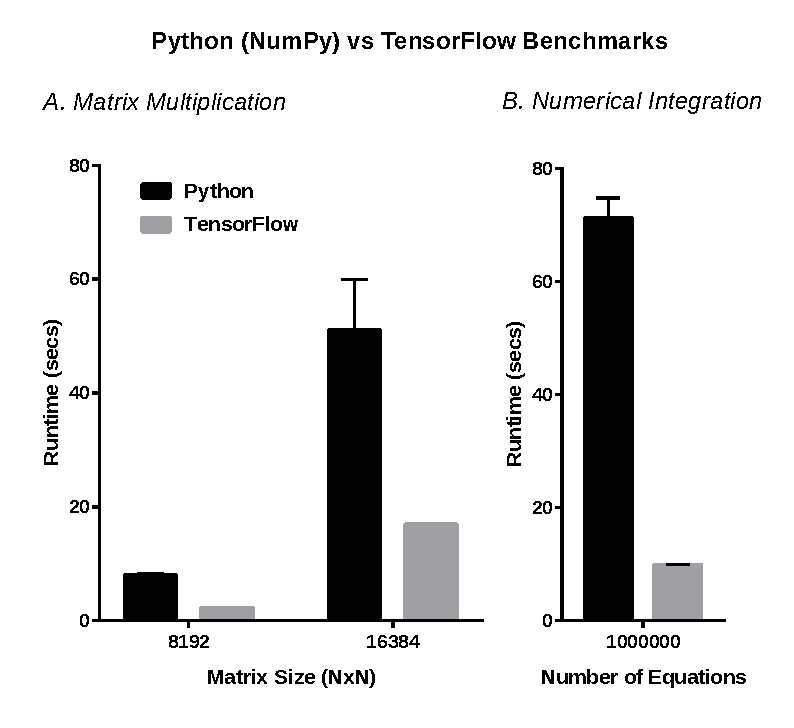
\includegraphics[scale=0.7]{Figures/Bench.pdf} 
\caption{Comparison of Python and Tensorflow on an 8 core, 2.1GHz desktop with 2 Intel Xeon E5-2620 processors}
\label{fig:comparison}
\end{figure}

These tutorials were written to address the needs of a group of undergraduate students in our institute. These students came from diverse backgrounds and had a basic introduction to Python during their first semester. They were interested in working on problems in Computational Neuroscience. Our goal was to introduce them to some of the numerical tools and mathematical models in Neuroscience while also allowing them to tinker with advanced projects that required writing code that ran on distributed systems. We were careful to keep the innards of the code visible \textemdash the form of the integrator, the specification of the differential equations and the ability to modify the code to suit their needs was particularly important. Towards the end of the tutorial, that many students managed to devour within a day or two, they were in a position to write codes simulating networks of neurons in the antennal lobe  \cite{Bazhenov2001}  (the insect equivalent of the olfactory bulb in mammals), firing rate models of grid cells~\cite{Burak2009}, detailed networks of stellate cells and inhibitory interneurons~\cite{Neru2019} and networks with plastic synapses~\cite{Bazhenov2005}. 

%~\cite{bib1}

\section*{How to use this Tutorial}
A reader familiar with Python will find this tutorial accessible. We use a number of Numpy (ref Numpy docs) and Matplotlib (ref Matplotlib docs) functions to simulate and display figures. These libraries are well documented with excellent introductory guides. During Day 1 of this tutorial we introduce numerical integration using Python without using any TensorFlow functions. On Day 2 we use TensorFlow functions to implement the integrator. Day 5 talks about memory management in TensorFlow. On Days 3 and 4 we use the code developed on Days 1 and 2 to simulate networks of conductance based neurons. Readers who are interested in solving differential equations in other domains will find the tutorial on Days 1, 2 and 5 self-contained.  Our simulations were run on a Linux desktop running Ubuntu xx.xx and on Google Cloud. We recommend that readers install Python 3.6 or above, Jupyter Notebook, Numpy Python package~\cite{numpy}, Matplotlib Python package~\cite{matplotlib}, and TensorFlow 1.13 or above using the Anaconda distribution of Python 3. The tutorials are linked in the supplementary material as Python notebooks (.ipynb files) that can be accessed using Jupyter and as .html files that can be read using any browser.
% For figure citations, please use "Fig" instead of "Figure". Fig~\ref{fig1}

% Place figure captions after the first paragraph in which they are cited.
%\begin{figure}[!h]
%\caption{{\bf Bold the figure title.}
%Figure caption text here, please use this space for the figure panel descriptions instead of using subfigure commands. A: Lorem ipsum dolor sit amet. B: Consectetur adipiscing elit.}
%\label{fig1}
%\end{figure}

\section*{Day 1: Solving ODEs using Python}
In this tutorial we are interested in solving ordinary differential equations (ODEs) of the form,
\begin{equation}
\frac{dx}{dt} = f(x, t)
\label{eq:ode}
\end{equation}
where, $x$ is an $N-$dimensional vector and $t$ typically stands for time. The function $f(x,t)$ may be a nonlinear function of $x$ that explicitly depends on $t$. In addition to specifying the form of the differential equation, one must also specify the value of $x$ at a particular time point. Say, $x=x_{0}$ at $t = t_0$. It is often not possible to derive a closed form solution for the equation(\ref{eq:ode}). Therefore numerical methods to solve these equations are of great importance. One example of ODEs at the core of our tutorial are the Hodgkin-Huxley equations describing the dynamics of action potential generation and propagation in the giant axon of the squid~\cite{Huxley1952}. Alan Hodgkin and Andrew Huxley arrived at these equations after a series of clever experiments that tested the limits of experimental technology available at the time. It also tested the limits of computational tools available. The form of the differential equations they derived contained nonlinearities that made it analytically intractable. In order to compute action potentials, Huxley numerically intergrated the equations using a hand operated Bunsviga mechanical calculator. The calculation took nearly three weeks to complete~\cite{Hodgkin1976}. They used a numerical method due to (see numerical methods section in \cite{Hodgkin1976}) to integrate the differential equations. Each iteration that calculated the value of the solution at subsequent time points consisted of 9 steps. In calculating the solution over time, they also varied the step size such that dynamics occurring over faster time scales (such as the rising phase of the action potential) were calculated with time step sizes of $0.1-0.2$ms while slower dynamics (such as the small highly damped oscillation following a spike) was calculated with time steps that were an order of magnitude higher ($1$ms).

In this tutorial, we illustrate two numerical methods to iteratively compute each time step of the solution. The first is a simple one-step method known as the Euler's method of integration. The second is another popular method, the Runge-Kutta method of order 4 (abberviated as RK4) that is more accurrate than the Euler's method, but requires additional computations to calculate the value of the solution at each time step. There are several textbooks on numerical methods. For the integrators described here, we have used~\cite{kreyszig1983}

\subsection*{Euler's Method for Numerical Integration}
Our goal is to solve (\ref{eq:ode}) - calculate $x(t)$ given an initial condition $x(t_n)=x_{n}$. The simplest method to solve (\ref{eq:ode}) numerically is the Euler's method. Here we start from $x(t=t_{0})=x_{0}$ and compute the solution at subsequent time points ($t_{0}+\epsilon,t_{0}+2\epsilon,t_{0}+3\epsilon \dots $) iteratively. Each step of the computation is done using the same formula that can be derived by truncating a Taylor series after the first term. That is, the solution at time $t_{0}+\epsilon$ is given by,
\begin{equation}
x(t_{0}+\epsilon) = x_{t){0}} + \epsilon\frac{dx}{dt} + \mathcal{O}(\epsilon^2)
\label{eq:euler}
\end{equation}
where $\frac{dx}{dt}=f(x,t)$. The higher order terms $\mathcal{O}(\epsilon^2)$ are ignored in this approximation. 

\begin{figure}[H]
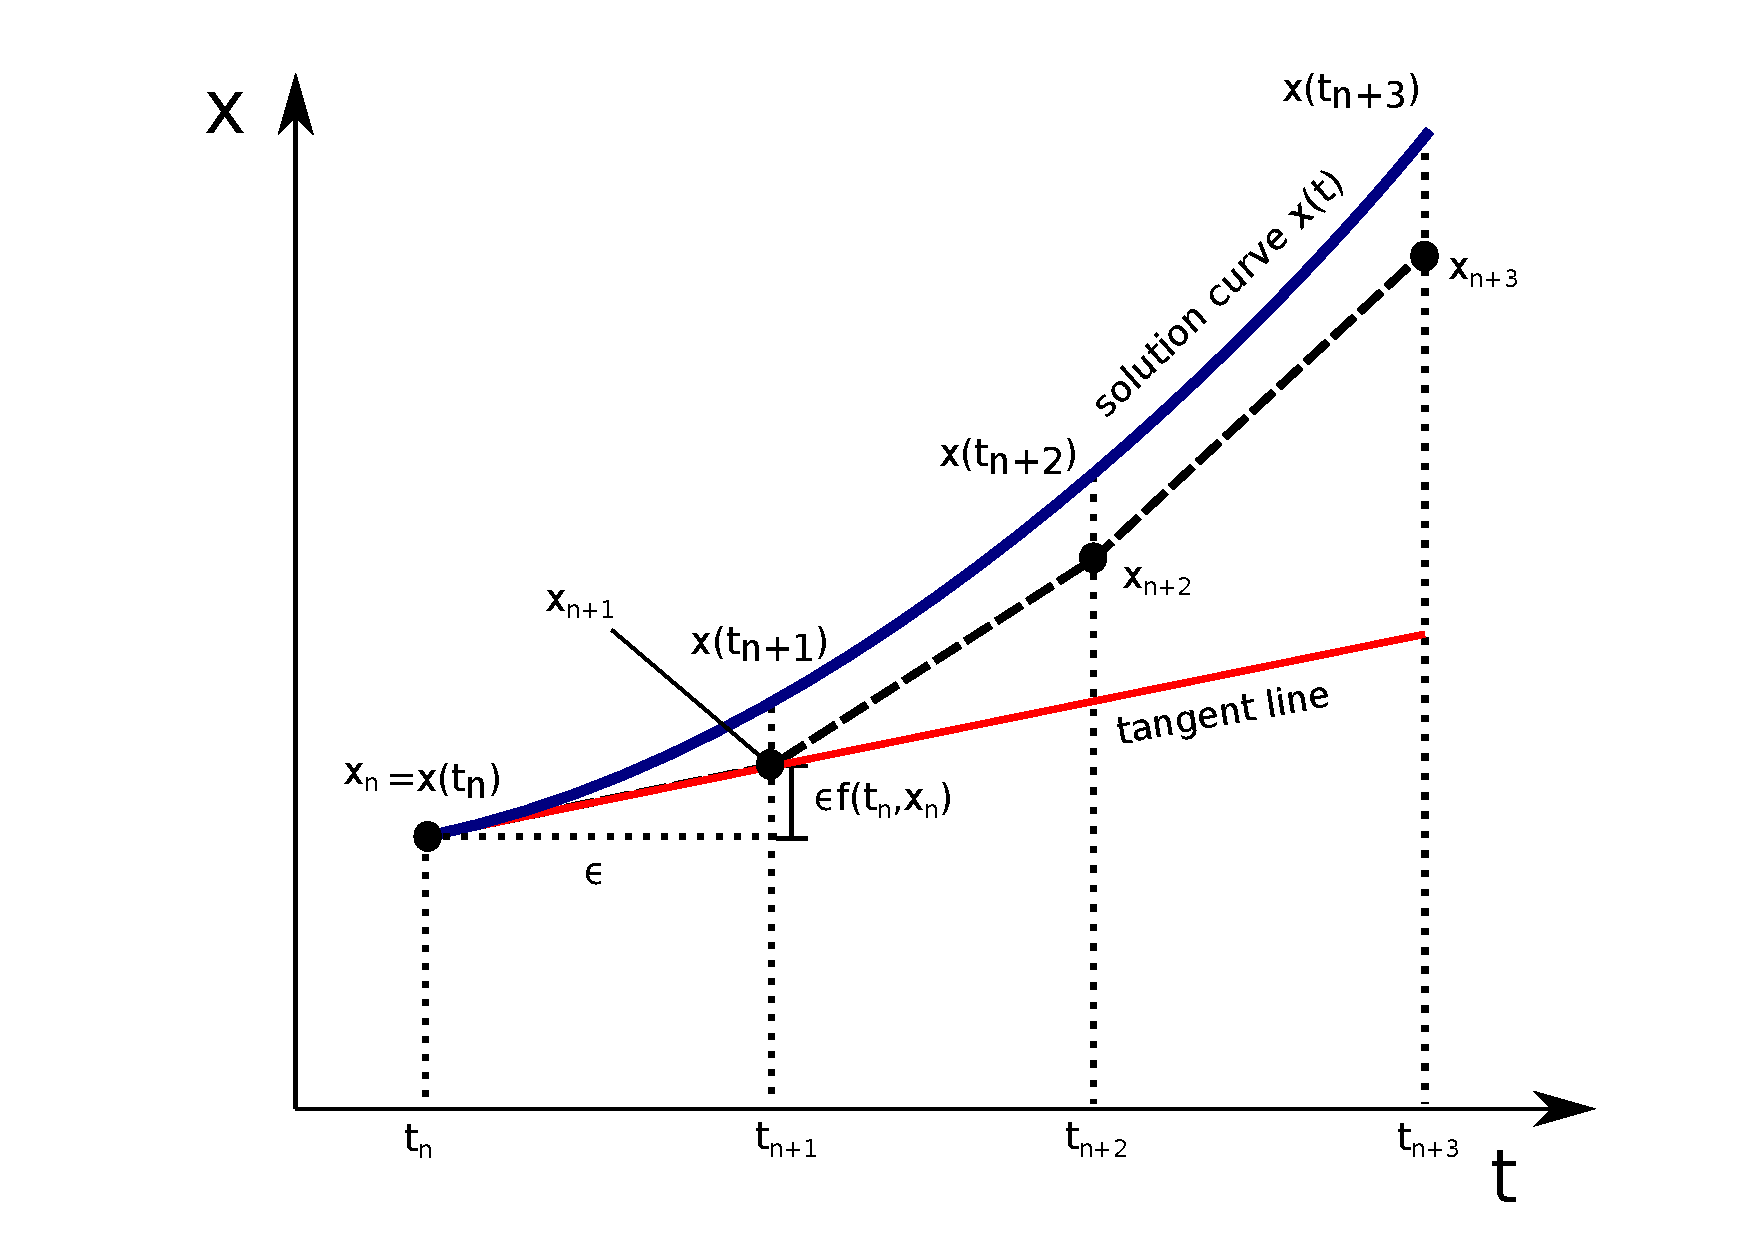
\includegraphics[scale=0.4]{Figures/fig1.pdf} 
\caption{Euler's method}
\label{fig:euler}
\end{figure}

A geometric interpretation of the Euler's method is shown in figure~\ref{fig:euler}. The solution of a particular differential equation is represented by the solid blue line in the figure. The dashed line approximates this solution by iteratively calculating $x$ at different time points using equation~\ref{eq:euler}. If the value of the solution at $t_{n}$ is $x_{n}$, $f(x_{n},t)$ is the slope of the tangent to the solution at $t_{n}$. If $\epsilon$ is sufficiently small, the solution at $t_{n+1}=t_{n}+\epsilon$ can be approximated by linearly extrapolating from $x_{n}$ to $x_{n} + \epsilon f(x_{n},t_{n})$

\subsection*{Implementation of Euler's Method in Python}

Let $\frac{dx}{dt}=5x$. We wish to calculate $x(t)$ over the interval $t\in[0,2)$  given the initial condition $x(0)=1$. The exact solution of this equation is $x(t) = e^{5t}$. In our implementation of Euler's method, we used the Python library Numpy to create and operate on arrays, and the plotting library Matplotlib, to display the results. We implement Euler's Method in Python as follows:

\begin{minted}[linenos]{python}
import numpy as np
import matplotlib.pyplot as plt
def f(x,t): # define the function f(x,t)
    return 5*x
epsilon = 0.01 # define timestep
t = np.arange(0,2,epsilon) # define an array for t
x = np.zeros(t.shape) # define an array for x
x[0]= 1 # set initial condition
for i in range(1,t.shape[0]):
    x[i] = epsilon*f(x[i-1],t[i-1])+x[i-1] # Euler Integration Step
\end{minted}

\begin{figure}[H]
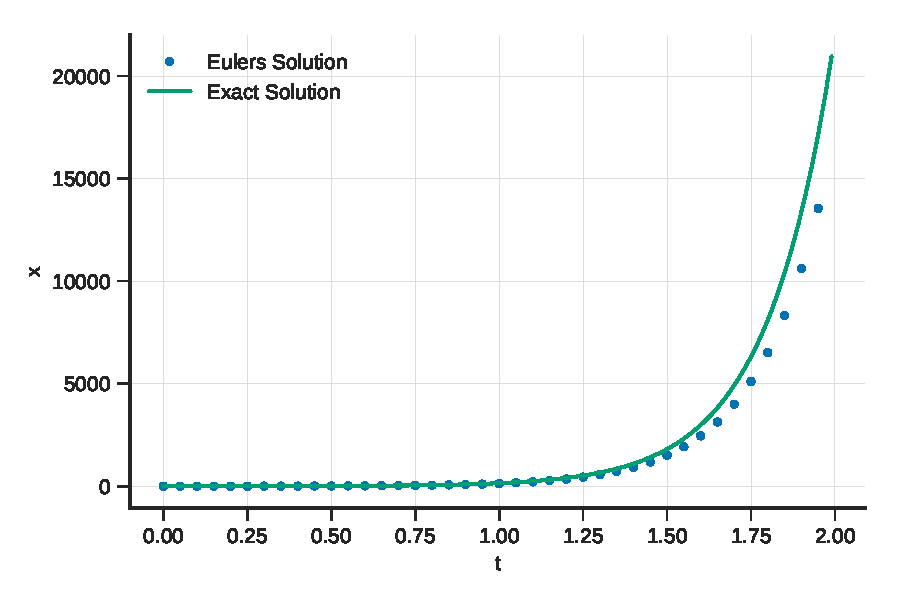
\includegraphics[scale=0.7]{Figures/fig2.pdf} 
\caption{Comparison of actual solution and approximation by Euler's method}
\label{fig:eulerError}
\end{figure}

The exact solution and the numerical solution are compared in Fig~\ref{fig:eulerError}. Notice that the approximation begins to diverge from the actual solution of the equation as the number of iterations increase. The omission of terms $\mathcal{O}(\epsilon^2)$ leads to a truncation error per step that can accumulate over time. 

\subsection*{Implementing Euler's method to solve a system of differential equations}

The implementation above can be easily extended to systems of equations. The Initial Value problem now becomes:

\begin{eqnarray}\frac{d\vec{X}}{dt} = \vec{f}(\vec{X}, t)\end{eqnarray}
\begin{eqnarray}\vec{X}(t_o) = \vec{X_o}\end{eqnarray}

where $\vec{X}=[X_1,X_2...]$ and $\vec{f}(\vec{X}, t)=[f_1(\vec{X}, t),f_2(\vec{X}, t)...]$. We rewrite Euler's method as:

\begin{eqnarray}t_{n+1} = t_n + \epsilon \end{eqnarray}
\begin{eqnarray}\vec{X}(t_{n+1}) = \vec{X}(t_{n}) + \epsilon \vec{f}(\vec{X}(t_{n}), t_n)\end{eqnarray}

Let $\frac{d\vec{X}}{dt}=f(\vec{X},t)$, we wish to find $\vec{X}(t)$ over $t\in[0,2)$, given that $\vec{X}(t)=[x,y]$, $\vec{X}(0)=[1,0]$ and $f(\vec{X},t) = [x-y,y-x]$. We implement the modified algorithm as follows:

\begin{minted}[linenos]{python}
def f(X,t): # the function f(X,t) now takes a vector X as input
    x,y = X #the first and the second elements of X are assigned to x and y
    return np.array([x-y,y-x])
t = np.arange(0,2,epsilon) # define an array for t
X = np.zeros((2,t.shape[0])) # initialize an array for X
X[:,0]= [1,0] # set initial condition
for i in range(1,t.shape[0]):
    X[:,i] = epsilon*f(X[:,i-1],t[i-1])+X[:,i-1] # Euler Integration Step
\end{minted}

\subsection*{A generalized code to the Euler method}
Here we rewrite the code in a modular fashion and cast the integrator as a function that takes in 3 inputs ie. the function $\vec{f}(\vec{y},t)$ where $\frac{d\vec{y}}{dt}=f(\vec{y},t)$, the time array, and initial vector $\vec{y}_{0}$. We will find this form to be particularly useful when we use TensorFlow functions to code the integrator. Further, it allows us to write multiple integrating functions (for example Euler or RK4) within the same class and call a specific integrator as needed. In addition we also introduce a function to ensure that the correct inputs are given to the integrator failing which an error message is generated. 

\subsubsection*{Algorithm}

\begin{itemize}
\item Get the required inputs: function $\vec{f}(\vec{y},t)$, initial condition vector $\vec{y}_0$ and time series $t$. Entering a time series $t$ allows for greater control over $\epsilon$ as it can now vary for each timestep. 
\item Check if the input is of the correct datatype ie. floating point decimal.
\item Create a zero matrix to hold the output.
\item For each time step, perform the update $\vec{y}$ using the Euler method with variable $\epsilon$ and store it in the output matrix.
\item Return the output time series [number of equations $\times$ iterations] matrix.
\end{itemize}

\begin{minted}[linenos]{python}
def check_type(y,t): # Ensure Input is Correct
    return y.dtype == np.floating and t.dtype == np.floating
class _Integrator():
    def integrate(self,func,y0,t):
        time_delta_grid = t[1:] - t[:-1]
        y = np.zeros((y0.shape[0],t.shape[0]))
        y[:,0] = y0
        for i in range(time_delta_grid.shape[0]):
            y[:,i+1]= time_delta_grid[i]*func(y[:,i],t[i])+y[:,i]
        return y
def odeint_euler(func,y0,t):
    y0 = np.array(y0)
    t = np.array(t)
    if check_type(y0,t):
        return _Integrator().integrate(func,y0,t)
    else:
        print("error encountered")
solution = odeint_euler(f,[1.,0.],t)
\end{minted}

\subsection*{Runge-Kutta Methods for Numerical Integration}

Euler's method $x_{n+1}=x_n + \epsilon f(x_n,t_n)$ calculates the solution at $t_{n+1}=t_n+\epsilon$ given the solution at $t_n$. In doing so we use the derivative at $t_{n}$ though its value may change throughout the interval $[t,t+\epsilon]$.  This results in an error in the order of $\mathcal{O}(\epsilon^2)$. By calculating the derivatives at intermediate steps, one can reduce the error at each step. Consider the following second order method where the slope is calculated at $t_{n}$ and $t_n+\frac{\epsilon}{2}$.

\begin{eqnarray}k_1=\epsilon f(x_n,t_n)\end{eqnarray}
\begin{eqnarray}k_2=\epsilon f(x_n+\frac{k_1}{2},t_n+\frac{\epsilon}{2})\end{eqnarray}
\begin{eqnarray}x_{n+1}=x_n+k_2+O(\epsilon^3)\end{eqnarray}


This method is called the second order Runge-Kutta method or the midpoint method.
\begin{figure}
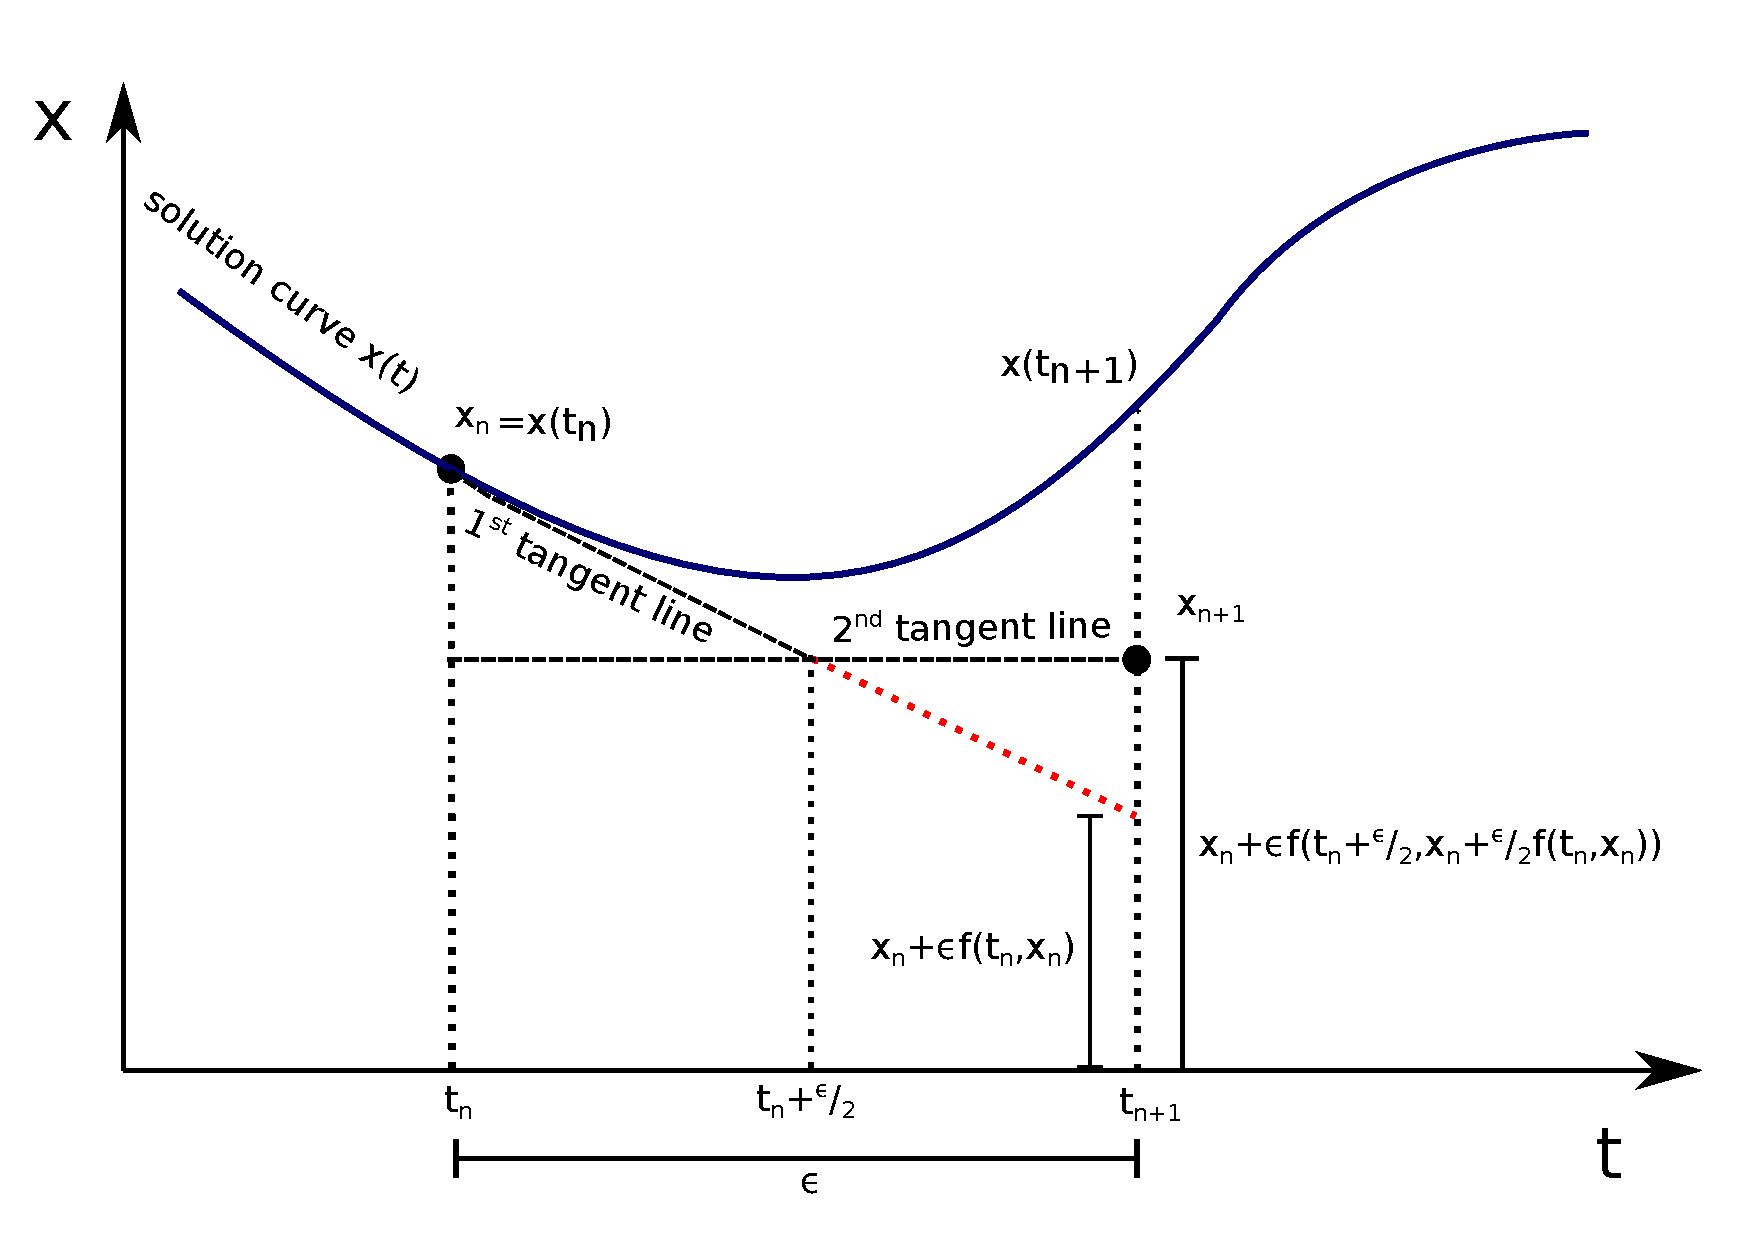
\includegraphics[scale=0.4]{Figures/fig4.pdf} 
\caption{Second order Runge-Kutta method}
\label{fig:RK2}
\end{figure}
Figure~\ref{fig:RK2} is a schematic description of the second order Runge-Kutta method. The blue curve denotes a solution of some differential equation. 

We can reduce errors by calculating additional derivatives. One of the most commonly used integrators is the fourth-order Runge-Kutta Method or RK4 method, that is implemented below:

\begin{eqnarray}k_1=f(x_n,t_n)\end{eqnarray}
\begin{eqnarray}k_2=f(x_n+\epsilon\frac{k_1}{2},t_n+\frac{\epsilon}{2})\end{eqnarray}
\begin{eqnarray}k_3=f(x_n+\epsilon\frac{k_2}{2},t_n+\frac{\epsilon}{2})\end{eqnarray}
\begin{eqnarray}k_4=f(x_n+\epsilon k_3,t_n+\epsilon)\end{eqnarray}
\begin{eqnarray}y_{n+1}=y_n+\frac{\epsilon}{6}(k_1+2 k_2+2 k_3+k_4)+\mathcal{O}(\epsilon^5)\end{eqnarray}

Note that this numerical method is again easily converted to a vector algorithm by simply replacing $x_i$ by the vector $\vec{X_i}$. We will use this method to simulate networks of neurons.

\subsection*{Generalized RK4 Method in Python}

We can now modify the Euler Integration code implemented earlier with a generalized function for RK4 that takes three inputs \textemdash the function $f(\vec{y},t)$ when $\frac{d\vec{y}}{dt}=f(\vec{y},t)$, the time array, and an initial vector $\vec{y_0}$. The code can be updated as follows,

\begin{minted}[linenos]{python}
# RK4 Integration Steps replace the Euler's Updation Steps
k1 = func(y[:,i], t[i])                               
half_step = t[i] + time_delta_grid[i] / 2
k2 = func(y[:,i] + time_delta_grid[i] * k1 / 2, half_step)
k3 = func(y[:,i] + time_delta_grid[i] * k2 / 2, half_step)
k4 = func(y[:,i] + time_delta_grid[i] * k3, t + time_delta_grid[i])
y[:,i+1]= (k1 + 2 * k2 + 2 * k3 + k4) * (time_delta_grid[i] / 6) + y[:,i]
\end{minted}

As an \textbf{Exercise}, solve the equation of a simple pendulum and observe its dynamics using the Euler and RK4 methods. Change the time step ($\epsilon$) and compare the resulting solutions. The equation of motion of a simple pendulum is given by: 

\begin{eqnarray}\frac{d^2s}{dt^2}=L\frac{d^2\theta}{dt^2}=-g\sin{\theta}\end{eqnarray}

where $L$ = Length of String and $\theta$ = angle made with vertical. To solve this second order differential equation convert it to a system of first order ODEs using a variable $\omega$ that represents the angular velocity.

\begin{eqnarray}\frac{d\theta}{dt}=\omega \end{eqnarray}
\begin{eqnarray}\frac{d\omega}{dt}=-\frac{g}{L}\sin{\theta} \end{eqnarray}

\section*{Day 2: Let the Tensors Flow!}

\subsection*{An Introduction to TensorFlow}

TensorFlow is an open-source library that was developed by researchers and engineers in the Google Brain team. TensorFlow has a number of functions that make it particularly suitable for machine learning applications. However, it is primarily an interface for numerical computation~\cite {tensorflow2015-whitepaper}. All computations in TensorFlow are specified as directed graphs (nodes connected by arrows) known as data flow graphs. Nodes are operations such as addition, multiplication etc. The incoming edges for each node are tensors (scalars, vectors, matrices and higher dimensional arrays), the actual values that are operated upon. The output is also a tensor that results from the computation. For example, consider the following computation where two vectors $a$ and $b$ serve as inputs to the node, a matrix multiplication operation, that produces a matrix $c$ as output.

\begin{figure}[H]
\begin{center}
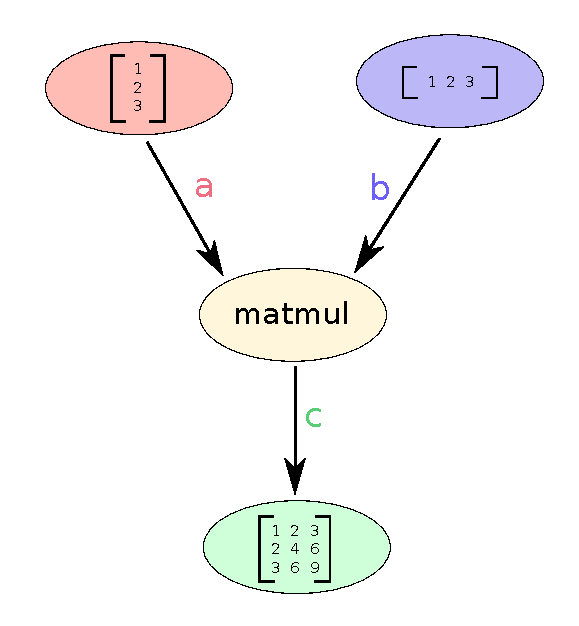
\includegraphics[scale=0.7]{Figures/fig6.pdf} 
\caption{Example of a simple computational graph}
\label{fig:compGraph}
\end{center}

\end{figure}
The following program implements the computation described in Figure(\ref{fig:compGraph}).

\begin{minted}[linenos]{python}
# Creating nodes in the computation graph 
a = tf.constant([[1.],[2.],[3.]], dtype=tf.float64) # a 3x1 column matrix 
b = tf.constant([[1.,2.,3.]], dtype=tf.float64) # a 1x3 row matrix 
c = tf.matmul(a, b) 
# To run the graph, we need to create a session.
# Creating the session initializes the computational device.
sess = tf.Session() # start a session
output = sess.run(c) # compute the value of c
sess.close() # end the session
print(output)
# TO automatically close the session after computation, Use:
# with tf.Session() as sess:
#    output = sess.run(c) 
\end{minted}
By specifying the computation graph we also specify the dependcies among the nodes. One can thus split the graph into smaller chunks or sub-graphs that can be independently computed by different devices that coordinate with each other. This makes it possible to develop programs that are device independent and scalable across CPUs, GPUs , TPUs and clusters of servers. 

\subsection*{Efficient recursion with TensorFlow}
Numerical integration is essentially a recursive process over a time array $[t_{0},t_{1},t_{2},\dots t_{n}]$. The rules to update both the Euler and the RK4 integrators can be written as a recursive function $F$ such that $X_{i+1}=F(X_i,t_i,\epsilon_i)$. The solution of the differential equation is the array $[X_0,F(X_0,t_0,\epsilon_0),F(F(X_0,t_0,\epsilon_0),t_1,\epsilon_1)...]$. We us the TensorFlow function \texttt{tf.scan} ~\cite{tensorflow-api-docs} to iterate over the time array. The arguments of \texttt{tf.scan} are a (i)a recursive function (ii)the list to iterate over and (iii)the initial value. If the initial value is not specified \texttt{tf.scan} uses the first element of the list as an initializer. As an example, consider the following program that  calculates the cumulative sum over a list. Every step involves adding an element from the list onto the last addition. 

\begin{minted}[linenos]{python}
# define the recursive function that takes in two values the
# accumulated value and the additional input from a list.
def recursive_addition(accumulator,new_element):
    return accumulator+new_element
# define the list over which we iterate
elems = np.array([1, 2, 3, 4, 5, 6])
# tf.scan takes in three inputs: the recursive function, the 
# list to iterate over and the initial value. If an initial 
# value is not provided, its taken as the first element of elems.
# accumulate with no initializer
cum_sum_a = tf.scan(recursive_addition, elems) 
# accumulate with initializer as the number 5
cum_sum_b = tf.scan(recursive_addition, elems, tf.constant(5,dtype=tf.int64))
with tf.Session() as sess:
    output_a = sess.run(cum_sum_a)
    output_b = sess.run(cum_sum_b)
print(output_a)
print(output_b)
# This prints :
#[ 1  3  6 10 15 21]
#[ 6  8 11 15 20 26]
\end{minted}

\textbf{Exercise} Use \texttt{tf.scan} to compute the Fibonacci sequence. 

\subsection*{Euler Integration Function with TensorFlow}
We now implement Euler's method using \texttt{tf.scan} to iterate over the time array. Note that the function \texttt{scan\_func} that defines each step of Euler's method, is now an input to \texttt{tf.scan}.

\begin{minted}[linenos]{python}
def tf_check_type(t, y0): # Ensure Input is Correct
    if not (y0.dtype.is_floating and t.dtype.is_floating): 
        # The datatype of any tensor t is accessed by t.dtype
        raise TypeError('Error in Datatype')
class _Tf_Integrator():
    def integrate(self, func, y0, t): 
        time_delta_grid = t[1:] - t[:-1]  
        def scan_func(y, t_dt): 
            t, dt = t_dt
            dy = dt*func(y,t)
            return y + dy
        # iterating over (a,b) where a and b are lists of same size
        # results in the ith accumulative step in tf.scan receiving
        # the ith elements of a and b zipped together
        y = tf.scan(scan_func, (t[:-1], time_delta_grid),y0) 
        return tf.concat([[y0], y], axis=0)
def tf_odeint_euler(func, y0, t):
    # Convert input to TensorFlow Objects
    t = tf.convert_to_tensor(t, preferred_dtype=tf.float64, name='t')
    y0 = tf.convert_to_tensor(y0, name='y0')
    tf_check_type(y0,t)
    return _Tf_Integrator().integrate(func,y0,t)
    
# Define a function using Tensorflow math operations. 
# This creates the computation graph.
def f(X,t):
    # extracting a single value eg. X[0] returns a single value but
    # we require a tensor, so we extract a range with one element.
    x = X[0:1] 
    y = X[1:2]
    out = tf.concat([x-y,y-x],0)
    return out
y0 = tf.constant([1,0], dtype=tf.float64)
epsilon = 0.01
t = np.arange(0,2,epsilon)
# Define the final value (output of scan) that we wish to compute
state = tf_odeint_euler(f,y0,t)
# Start a TF session and evaluate state
with tf.Session() as sess:
    state = sess.run(state)
\end{minted}

\subsection*{RK4 Integration Function with TensorFlow}

Now, we implement the RK4 integrator. Note that here we replace the single step iterator used for the Euler's with a four step RK4 iterator. In addition, to make the code more modular, we define a function \texttt{\_step\_func()} that is called by \texttt{scan\_func} and calculates the next step of the RK4 integrator. The rest of the program remains the same as the Euler's method implemented above.

\begin{minted}[linenos]{python}
def integrate(self, func, y0, t): 
        time_delta_grid = t[1:] - t[:-1]
        def scan_func(y, t_dt): 
            t, dt = t_dt
            dy = self._step_func(func,t,dt,y) # Make code more modular.
            return y + dy
        y = tf.scan(scan_func, (t[:-1], time_delta_grid),y0)
        return tf.concat([[y0], y], axis=0)
    def _step_func(self, func, t, dt, y):
        k1 = func(y, t)
        half_step = t + dt / 2
        dt_cast = tf.cast(dt, y.dtype) # Failsafe
        k2 = func(y + dt_cast * k1 / 2, half_step)
        k3 = func(y + dt_cast * k2 / 2, half_step)
        k4 = func(y + dt_cast * k3, t + dt)
        return tf.add_n([k1, 2 * k2, 2 * k3, k4]) * (dt_cast / 6)
\end{minted}

\textbf{Exercise}, Simulate the non-linear Lorentz Attractor using the Euler and RK4 with TensorFlow. The equations of the Lorenz Attractor are given by,

\begin{eqnarray}\frac{dx}{dt}=\sigma(y-x) \end{eqnarray}
\begin{eqnarray}\frac{dy}{dt}=x(\rho-z)-y \end{eqnarray}
\begin{eqnarray}\frac{dz}{dt}=xy-\beta z \end{eqnarray}

Use the values $\sigma =10$, $\beta =\frac{8}{3}$, $\rho =28$. Simulate these equations for similar initial conditions and compare how the trajectories diverge. The solution of the Lorenz equations should resemble Figure~\ref{fig:Lorenz}
 
\begin{figure}[H]
\begin{center}
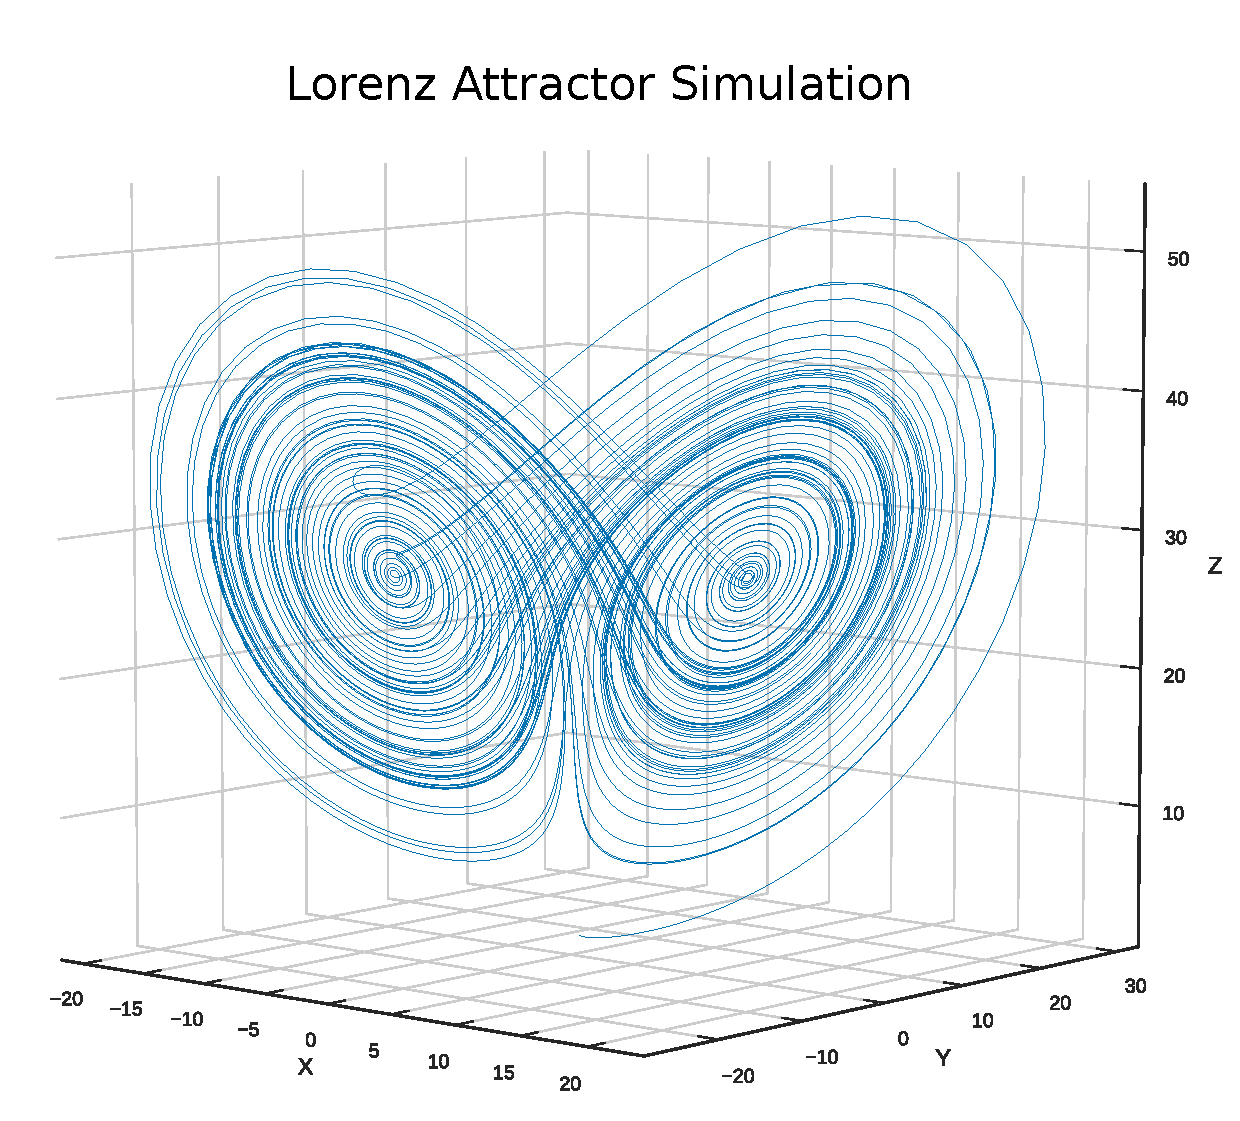
\includegraphics[scale=0.5]{Figures/fig6_op.pdf} 
\caption{Example of a simple computational graph}
\label{fig:Lorenz}
\end{center}

\end{figure}

\section*{Day 3: Neurons in Silicon}
The electric potential measured across the membranes of excitable cells, such as neurons or heart cells, can undergo transient changes when perturbed by external inputs. When the inputs to a neuron are sufficiently large these transient changes can regeneratively build up into a large deviation from the resting state known as an action potential. Action potentials propagate undiminished along the axon and perturb post-synaptic neurons. The Hodgkin-Huxley model is a system of differential equations that describe the generation an action potential and its propagation along the axon. We provide only a brief overview of the Hodgkin-Huxley model. A number of classic references~\cite{Dayan2005, Johnston1995} and the original papers by Hodgkin and Huxley~\cite{Huxley1952} chronicle the history and the details of the model. An excellent set of MOOCS ~\cite{gerstnerMOOC, compneuroMOOC} and the accompanying textbooks ~\cite{Gerstner2014,Dayan2005} give an accessible introduction to the topic

\subsection*{What is the Hodgkin Huxley Neuron Model?}
The cell membrane, a 5nm thick lipid bilayer, separates the inside from the outside of the neuron. The membrane is largely impermeable to charged ions present on either side. The concentration of Na\textsuperscript{+} ions outside the cell is greater than its concentration inside, while K\textsuperscript{+} ions are relatively abundant inside compared to the outside. In addition to these there are chloride (Cl\textsuperscript{-}), calcium (Ca\textsuperscript{2+}) and magnesium ions (Mg\textsuperscript{+}) that populate the cellular milieu. The differences in ionic abundances across the membrane cause a net accumulation of positive ions on one side of the membrane and negative ions on the other, and thus a potential difference across the membrane. Embedded on the membrane are ion channels that are highly selective to the ion species it lets across. In the squid axon, Hodgkin and Huxley found that there were only two types of ion channels (Na\textsuperscript{+} and K\textsuperscript{+}), in addition to a non-specific leak channel. The Hodgkin-Huxley model of neurons can be understood with the help of an equivalent electrical circuit Figure(\ref{fig:HH}) The cell membrane acts as a capacitor. An total injected current ($I$) can be written as the sum of the capacitive current $I_{C}$, ionic currents $I_{Na}$ and $I_{K}$ and the leak current $I_L$.

\begin{figure}[H]
\begin{center}
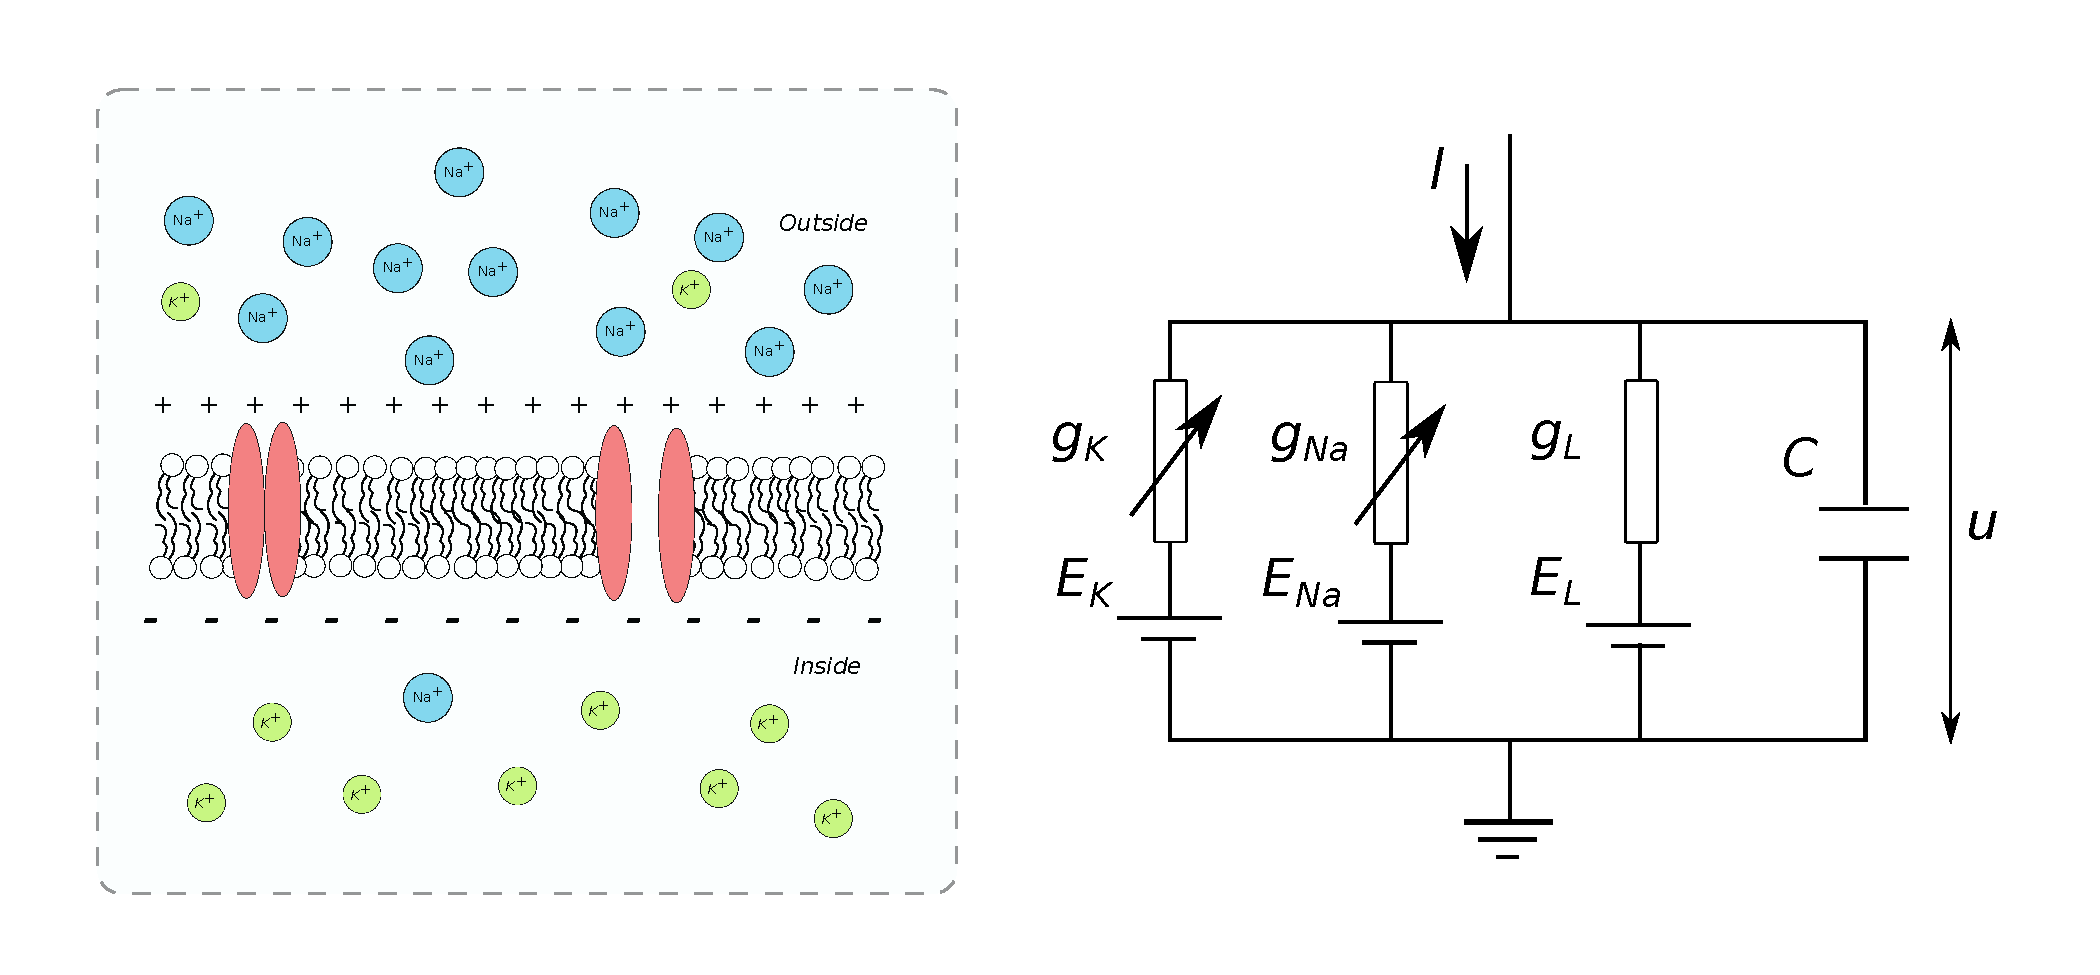
\includegraphics[scale=0.4]{Figures/fig7.pdf} 
\caption{HH Neuron}
\label{fig:HH}
\end{center}
\end{figure}

\begin{equation}
I = I_{C}(t) + I_{Na}(t) + I_{K}(t)
\end{equation}
where, 
\begin{eqnarray}
C_m = 1 \mu F/cm^2 \\
I_{Na} = g_{Na}(u-E_{Na})\\
I_{K} = g_{k}(u-E_K)\\
I_{L} = g_{L}(u-E_L)
\end{eqnarray}
The equation describing the membrane potential can thus be written as follows,
\begin{eqnarray}
\label{eq:HH}
C_m\frac{du}{dt}=−I_{Na}(t)−I_{K}(t)−I_{L}(t)+I(t)
\end{eqnarray}
Hodgkin and Huxley discovered that the $Na$ and the $K$ channels do not act as Ohmic conductances, but are modulated by the potential across the membrane. 
Changes in potential had a nonlinear effect on flow of ionic currents. Based in their experimental results they obtained a system of differential equations that described the temporal evolution of the membrane potential in terms of changes in ionic currents (chiefly Na\textsuperscript{+} and K\textsuperscript{+}). 

\begin{eqnarray}\label{d3_2}I_{Na} = g_{Na}m^3h(u−E_{Na})\end{eqnarray}
\begin{eqnarray}\label{d3_3}I_K = g_Kn^4(u−E_K)\end{eqnarray}
\begin{eqnarray}\label{d3_4}I_L = g_L(u−E_L)\end{eqnarray}

where $E_{Na}=50\ mV$, $E_K = -95\ mV$ and $E_L=-55\ mV$ are the reversal potentials; $g_{Na} = 100\ \mu S/cm^2$, $g_K = 10\ \mu S/cm^2$ and $g_L = 0.15\ \mu S/cm^2$ are the channel conductances; and m,h, and n are gating variables that follow the dynamics given by:

\begin{eqnarray}\label{d3_5}\frac{dm}{dt} = - \frac{1}{\tau_m}(m-m_0)\end{eqnarray}
\begin{eqnarray}\label{d3_6}\frac{dh}{dt} = - \frac{1}{\tau_h}(h-h_0)\end{eqnarray}
\begin{eqnarray}\label{d3_7}\frac{dn}{dt} = - \frac{1}{\tau_n}(n-n_0)\end{eqnarray}

where $\tau_m$, $\tau_h$ and $\tau_n$ are empirically determined voltage dependent time constants and $m_0$, $h_0$ and $n_0$ are voltage dependent asymptotic gating values.

\subsection*{Implementing the Hodgkin-Huxley neuron model}

The variable of the Hodgkin Huxley neuron model has that are updated at each integration time step are, the membrane potential, $V$, the sodium activation gating Variable, $m$, the sodium inactivation gating Variable, $h$, and the potassium channel gating Variable, $n$. The dynamics are given by Eq~(\ref{d3_5}),Eq~(\ref{d3_6}) and Eq~(\ref{d3_7}). In the following code, we define the parameters associated with the conductances, including the formulae for $\tau_{m}$, $\tau_{h}$, $\tau_{n}$ and the voltage dependent steady state values of the gating variables. 

\begin{minted}[linenos]{python}
# Step 1: Defining Parameters of the Neuron 
C_m = 1
g_K = 10
E_K = -95
g_Na = 100
E_Na = 50 
g_L = 0.15
E_L = -55
# Step 2: Defining functions to calculate tau_x and x_0
# Note: Always use TensorFlow functions for all operations.
def K_prop(V):
    T = 22
    phi = 3.0**((T-36.0)/10)
    V_ = V-(-50)
    alpha_n = 0.02*(15.0 - V_)/(tf.exp((15.0 - V_)/5.0) - 1.0)
    beta_n = 0.5*tf.exp((10.0 - V_)/40.0) 
    t_n = 1.0/((alpha_n+beta_n)*phi)
    n_0 = alpha_n/(alpha_n+beta_n)
    return n_0, t_n
def Na_prop(V):
    T = 22
    phi = 3.0**((T-36)/10)
    V_ = V-(-50)
    alpha_m = 0.32*(13.0 - V_)/(tf.exp((13.0 - V_)/4.0) - 1.0)
    beta_m = 0.28*(V_ - 40.0)/(tf.exp((V_ - 40.0)/5.0) - 1.0)
    alpha_h = 0.128*tf.exp((17.0 - V_)/18.0)
    beta_h = 4.0/(tf.exp((40.0 - V_)/5.0) + 1.0)
    t_m = 1.0/((alpha_m+beta_m)*phi)
    t_h = 1.0/((alpha_h+beta_h)*phi)
    m_0 = alpha_m/(alpha_m+beta_m)
    h_0 = alpha_h/(alpha_h+beta_h)
    return m_0, t_m, h_0, t_h
# Step 3: Defining function that calculate Neuronal currents
def I_K(V, n):
    return g_K  * n**4 * (V - E_K)
def I_Na(V, m, h):
    return g_Na * m**3 * h * (V - E_Na)
def I_L(V):
    return g_L * (V - E_L)
# Step 4: Define the function dX/dt where X is the State Vector
def dXdt(X, t):
    V = X[0:1]
    m = X[1:2]
    h = X[2:3]
    n = X[3:4]
    dVdt = (5 - I_Na(V, m, h) - I_K(V, n) - I_L(V)) / C_m 
    # Here the current injection I_injected = 5 uA
    m0,tm,h0,th = Na_prop(V)
    n0,tn = K_prop(V)
    dmdt = - (1.0/tm)*(m-m0)
    dhdt = - (1.0/th)*(h-h0)
    dndt = - (1.0/tn)*(n-n0)
    out = tf.concat([dVdt,dmdt,dhdt,dndt],0)
    return out
# Step 5: Define Initial Condition and Integrate
y0 = tf.constant([-71,0,0,0], dtype=tf.float64)
epsilon = 0.01
t = np.arange(0,200,epsilon)
state = odeint(dXdt,y0,t)
with tf.Session() as sess:
    state = sess.run(state)
\end{minted}

\subsection*{Simulating multiple independent Hodgkin-Huxley neurons}

Here we illustrate some simple steps that can be used to simulate populations of neurons efficiently. Key to setting up the equations is to order it in a manner that utilizes TensorFlow's algorithms that distribute vector, matrix and tensor computations over multiple cores. Consider a system of 20 independent HH neurons with different input currents that characterise the firing rates. 

\subsubsection*{Methods of Parallelization}
TensorFlow has built-in functions that speed up Tensor computations using available multi-cores, and GPU/TPU setups. There are two major parts of the code where such a speed-up can be effected
\begin{enumerate}
\item \textbf{RK4 iterations} Our implementation of the integrator utilizes Tensors as inputs. 
\item \textbf{Functional Evaluations:} The form of the equations that describe the neuronal dynamics,  are common across neurons. Only the parameters for differ across neurons. This can be used to `vectorize' the equations.
\end{enumerate}

Say $\vec{X}=[V,m,n,h]$ is the state vector of a single neuron and its dynamics are defined using parameters $C_m,g_K,...E_L$ equations of the form: 

\begin{eqnarray}\frac{d\vec{X}}{dt} = [f_1(\vec{X},C_m,g_K,...E_L),f_2(\vec{X},C_m,g_K,...E_L)...f_m(\vec{X},C_m,g_K,...E_L)]\end{eqnarray}

We can convert these equations to a form in which all evaluations are done as vector calculations and NOT scalar calculations. Despite the parameters being different, the functional forms of the equations are similar for the same state variable of different neurons. Thus, the trick is to reorganize $\mathbf{X}$ as $\mathbf{X'}=[(V_1,V_2,...V_n),(m_1,m_2,...m_n),(h_1,h_2,...h_n),(n_1,n_2,...n_n)]=[\vec{V},\vec{m},\vec{h},\vec{n}]$. And the parameters as $[\vec{C_m},\vec{g_K}] = [C_{m_{1}}\dots C_{m_{n}},g_{K_{1}}\dots g_{K_{n}}]$ and so on.

The advantage of this re-ordering is that the differential equation of the form,
\begin{eqnarray}\frac{dV_i}{dt}=f(V_i,m_i,h_i,n_i,C_{m_i},g_{K_i}...)\end{eqnarray}

is now easily parallelizable using a vector computation of the form, 

\begin{eqnarray}\frac{d\vec{V}}{dt}=f(\vec{V},\vec{m},\vec{h},\vec{n},\vec{C_m},\vec{g_K}...)\end{eqnarray}

The equations can now be written in the form,
\begin{eqnarray}\frac{d\mathbf{X'}}{dt}= \Big[\frac{d\vec{V}}{dt},\frac{d\vec{m}}{dt},\frac{d\vec{h}}{dt},\frac{d\vec{n}}{dt}\Big]\end{eqnarray}

\subsubsection*{Implementation}

Notice that the functions calculating the gating dynamics and channel currents are already capable of vector input and output, so we do not need to change these. However, the parameters were not defined as vectors in our earlier implementation.

\begin{minted}[linenos]{python}
n_n = 20 # number of simultaneous neurons to simulate
# parameters will now become n_n-vectors
C_m = [1.0]*n_n
g_K = [10.0]*n_n
E_K = [-95.0]*n_n
g_Na = [100]*n_n
E_Na = [50]*n_n 
g_L = [0.15]*n_n
E_L = [-55.0]*n_n

# The state vector definition will change
def dXdt(X, t):
    V = X[:1*n_n]       # First n_n values are Membrane Voltage
    m = X[1*n_n:2*n_n]  # Next n_n values are Sodium Activation Gating
    h = X[2*n_n:3*n_n]  # Next n_n values are Sodium Inactivation Gating
    n = X[3*n_n:]       # Last n_n values are Potassium Gating
    dVdt = (np.linspace(0,10,n_n)-I_Na(V, m, h)-I_K(V, n)-I_L(V))/ C_m 
    # Input current is linearly varied between 0 and 10
    m0,tm,h0,th = Na_prop(V)
    n0,tn = K_prop(V)
    dmdt = - (1.0/tm)*(m-m0)
    dhdt = - (1.0/th)*(h-h0)
    dndt = - (1.0/tn)*(n-n0)
    out = tf.concat([dVdt,dmdt,dhdt,dndt],0)
    return out
y0 = tf.constant([-71]*n_n+[0,0,0]*n_n, dtype=tf.float64)
\end{minted}
The firing frequency as a function of the input is shown in Figure(\ref{fig:freq}). The code to generate the firing rate is below.
\begin{center}
\begin{figure}
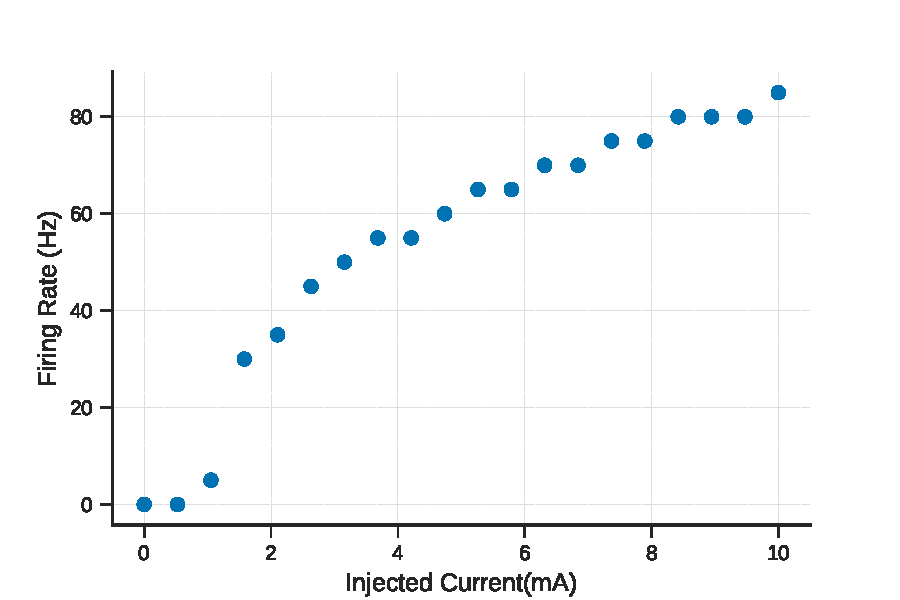
\includegraphics[scale=0.6]{Figures/fig12.pdf} 
\caption{ Firing frequency of the Hodgkin-Huxley neuron as a function of input amplitude}
\label{fig:freq}
\end{figure}
\end{center}

\begin{minted}[linenos]{python}
rate = np.bitwise_and(state[:-1,:20]<0,state[1:,:20]>0).sum(axis=0)/0.2
\end{minted}

\section*{Day 4: Neurons and Networks}
In this section we simulate a network of neurons interacting via synapses. Each synapse is defined by its own set of state variables and differential equations governing their temporal evolution. There are different kinds of synapses - electrical and chemical synapses. Electrical synapses are essentially physical conduits that allow the flow of ions across connected neurons. Chemical synapses are more common in the brain and are more complex than electrical synapses. When an action potential arrives at the axon terminal, it leads to the opening of voltage-gated calcium channels. The incoming calcium triggers neurotransmitter filled vesciles to fuse with the axon terminal membrane and release their cargo into the synaptic cleft. The neurotransmitters diffuse across the cleft and open (or close) ion channels on the post-synaptic neuron. This can cause a depolarization (increase in potential across the post-synaptic neuron's membrane) that makes it easier for the neuron to spike or it can inhibit the neuron and have the opposite effect. In some cases these effects are fast and direct \textemdash a neurotransmitter binds to a receptor in the post-synaptic site that causes an influx or efflux of ions and leads to a change in the membrane potential. The effect of a synapse can also be indirect such that neurotransmitters invoke a second messenger cascade that eventually leads to the opening or closing of ion channels in the post-synaptic neuron. Here we model fast excitatory and inhibitory chemical synapses.The network of interactions between neurons will be described by a connectivity matrix. Different connectivity matrices describe the interactions due to different types of synapses. 

\subsubsection*{Modelling Synapses}

The synaptic current ($I_{syn}$) depends on the difference between the reversal potential ($E_{syn}$) and the value of the membrane potential ($u$). The synaptic current due to neurotransmitter release into the synaptic cleft following an action potential is given by,
\begin{equation}
I_{syn}(t)=g_{syn}(t)(u(t)−E_{syn})
\label{eq:syncurr}
\end{equation}
When the transmitter binds to postsynaptic receptors it causes a transient change in the conductance $g_{syn}$. To capture the dynamics of $g_{syn}$, one models the system using a simple kinetic model where the receptors can be either in an open or a closed state~\cite{Destexhe1994}. The transition between the states is proportional to the concentration of the neurotransmitter $[T]$ in the cleft. 
\begin{equation}
\mathrm{C}\underset{\beta}{\stackrel{\alpha[T]}{\rightleftharpoons}} \mathrm{O}
\end{equation}
This may be rewritten in the form of a differential equation.
\begin{eqnarray}\label{d4_1}\frac{d[O]}{dt}=\alpha[T](1−[O])−\beta[O]\end{eqnarray}
We can now describe the synaptic conductance $g_{syn}(t)=g_{max}[O]$, in terms of the maximal conductance $g_{max}$ and a gating variable $[O]$, where $[O](t)$ is the fraction of open synaptic channels. $\alpha$ is the binding constant, $\beta$ the unbinding constant and $(1−[O])$ the fraction of closed channels where the neurotransmitter can bind. The functional form of T depends on the nature of the synapse.
For cholinergic excitatory synapses, $[T]$ is given by,
\begin{eqnarray}
\label{d4_2}
[T]_{ach} = A\ \Theta(t_{max}+t_{fire}+t_{delay}-t)\ \Theta(t-t_{fire}-t_{delay})
\end{eqnarray}
where, $\Theta (x)$ is the Heaviside step function, $t_{fire}$ is the time of the last presynaptic spike, $t_{delay}$ is the time delay from the time of the last spike to its effect on the postsynaptic neuron and $t_{max}$ is the duration after the spike during which the transmitter remains in the synaptic cleft.
For Fast GABAergic inhibitory synapses, we used the following equation,
\begin{eqnarray}\label{d4_3}[T]_{gaba} = \frac{1}{1+e^{-\frac{V(t-t_{fire}-t_{delay})-V_0}{\sigma}}}\end{eqnarray}

Note that in order to solve the equation~\ref{d4_1}, we need to determine the time when the presynaptic neuron fired ($t_{fire}$). To account for these synaptic interactions between neurons we need to modify the RK4 integrator developed to simulate multiple independent Hodgkin-Huxley neurons. 

\subsection*{Redesigning the Generalized TensorFlow Integrator}
In this section we modify the integrator that we coded on Day 2 to account for interactions between neurons. This will require an additional variable that stores the time elapsed from the last presynaptic spike to calculate the  equations~\ref{d4_2},~\ref{d4_3}. In the modified code we will use the TensorFlow function \texttt{tf.where()} to efficiently assign the indices of neurons that have spiked and those that have not spiked at each time point. To understand the usage and function of \texttt{tf.where()}, consider the following example. Say, you have a array \texttt{x} of 10 random numbers between 0 and 1. You want the output of the code to be another array of the same size as \texttt{x} such that the elements of the array are either -10 or 10 depending on whether the corresponding element in \texttt{x} is less or greater than 0.5. The function  \texttt{tf.where(cond,a,b)} outputs an array with elements from \texttt{a} if the condition \texttt{cond} is \texttt{True} and from \texttt{b} if \texttt{cond} is \texttt{False}. See the example code below.

\begin{minted}[linenos]{python}
# create the Tensor with the random variables
x = tf.constant(np.random.uniform(size = (10,)),dtype=tf.float64)
# a list of 10s to select from if true
if_true = tf.constant(10*np.ones((10,)),dtype=tf.float64)
# a list of -10s to select from if false
if_false = tf.constant(-10*np.ones((10,)),dtype=tf.float64)
# perform the conditional masking
selection = tf.where(tf.greater(x,0.5),if_true,if_false)
with tf.Session() as sess:
    x_out = sess.run(x)
    selection_out = sess.run(selection)
# If x_out = [0.13 0.08 0.58 0.17 0.34 0.58 0.97 0.66 0.30 0.29 ],
# selection_out = [-10. -10.  10. -10. -10.  10.  10.  10. -10. -10.]
\end{minted}

In order to determine whether a particular neuron fired, we introduce a new variable \texttt{fire\_t} that stores the time of the last spike for each neuron. 

We modify the code as follows:
\begin{enumerate}
\item The Integrator class that we defined earlier now requires two more properties as input, namely, the number of neurons (\texttt{n}) and firing threshold (\texttt{F\_b}) of each of these neurons. We provide these inputs as arguments to the Integrator class.
\item The state vector will now have an additional set of \texttt{n} variables representing the firing times. These will not be updated by the step function (\texttt{\_step\_func}).
\item Inside the Integrator class, we have access to the values of the state variable and the change in the state variable since the last iteration. We use this to check if the voltages have crossed the firing threshold. The convention followed in this code is, the first \texttt{n} elements of the state vector are the membrane voltages while the last \texttt{n} elements are the time from the last spike for each of the neurons.
\item The differential update function ie. step\_func takes except the last \texttt{n} values of the state variable and updates according to the differential equations specified in \texttt{func}. The last \texttt{n} variables are updated separately in \texttt{scan\_func}. It checks if any neuron has crossed its firing threshold and updates the variable \texttt{fire\_t} of the appropriate neurons with the current time.
\end{enumerate}

The modifications to the RK4 code implemented earlier is shown below,

\begin{minted}[linenos]{python}

def integrate(self, func, y0, t): 
        time_delta_grid = t[1:] - t[:-1]
        def scan_func(y, t_dt): 
            # recall the necessary variables
            n_ = self.n_
            F_b = self.F_b
            t, dt = t_dt
            # Differential updation
            dy = self._step_func(func,t,dt,y) # Make code more modular.
            dy = tf.cast(dy, dtype=y.dtype) # Failsafe
            out = y + dy # the result after differential updation
            # Use specialized Integrator vs Normal Integrator (n=0)
            if n_>0:
                # Extract the last n variables for fire times
                fire_t = y[-n_:] 
                # Change in fire_t if neuron didnt fire = 0
                l = tf.zeros(tf.shape(fire_t),dtype=fire_t.dtype) 
                # Change in fire_t if neuron fired = Current-Last Fire
                l_ = t-fire_t 
                # Check if previous Voltage is less than Threshold
                z = tf.less(y[:n_],F_b)              
                # Check if Voltage is more than Threshold after update
                z_ = tf.greater_equal(out[:n_],F_b)  
                df = tf.where(tf.logical_and(z,z_),l_,l) 
                fire_t_ = fire_t+df # Update firing time 
                return tf.concat([out[:-n_],fire_t_],0)
            else:
                return out
        y = tf.scan(scan_func, (t[:-1], time_delta_grid),y0)
        return tf.concat([[y0], y], axis=0)
        
def odeint(func, y0, t, n_, F_b):
    t = tf.convert_to_tensor(t, preferred_dtype=tf.float64, name='t')
    y0 = tf.convert_to_tensor(y0, name='y0')
    tf_check_type(y0,t)
    return _Tf_Integrator(n_, F_b).integrate(func,y0,t)
\end{minted}

\subsection*{Implementing a network of Hodgkin-Huxley neurons}

Recall, each Hodgkin Huxley Neuron in a network with $n$ neurons has 4 dynamical variables $V$, $ m$, $n$, $h$. Each of these variables were represented as $n$\textemdash dimensional vectors. Now we need to add some more state variables representing each synapse. The neuron receives excitatory and inhibitory inputs that are introduced as additional synaptic currents $I_{ach}$ and $I_{GABA}$. Equation~\ref{eq:HH} now reads, 

\begin{eqnarray}C_m\frac{dV}{dt} = I_{injected} - I_{Na} - I_K - I_L - I_{ach} - I_{gaba}\end{eqnarray}

For each synapse, we have Eq~(\ref{d4_1}), Eq~(\ref{d4_2}) and:

\begin{eqnarray}
\frac{d[O]_{ach/gaba}}{dt} = \alpha (1-[O]_{ach/gaba})[T]_{ach/gaba}-\beta[O]_{ach/gaba}
\label{eq:synO}
\end{eqnarray}

\begin{eqnarray}
I_{ach/gaba}(t)=g_{max}[O]_{ach/gaba}(V−E_{ach/gaba})
\label{eq:Isyn}
\end{eqnarray}

\subsection*{Synaptic Memory Management}

In a network with $n$ neurons, there are at most $n^2$ synapses of each type. The actual number may be much smaller. The dynamics of each synapse is given by the equation(\ref{eq:synO}). To illustrate the details of the implementation, consider the following three neuron network. Let $X_1$ be an excitatory neuron that forms a cholinergic synapse, $X_2$ an inhibitory neuron that extends a GABAergic synapse onto $X_3$. The network has the form: $X_1\rightarrow X_2\rightarrow X_3$. In defining the connectivity matrix for each synapse type, we set a convention where the presynaptic neurons are indexed by the column number, and the postsynaptic neurons by the row number. Let $X_1$, $X_2$, $X_3$ be indexed as 0, 1 and 2 respectively. The excitatory connectivity matrix takes the form

\begin{eqnarray}
Ach_{n\times n}=
\begin{bmatrix}
0&0&0\\
1&0&0\\
0&0&0\\
\end{bmatrix}
\end{eqnarray}

Similarly, the inhibitory connectivity matrix becomes

\begin{eqnarray}
GABA_{n\times n}=
\begin{bmatrix}
0&0&0\\
0&0&0\\
0&1&0\\
\end{bmatrix}
\end{eqnarray}

In the following code we specify the parameters of the synapse. The number of synapses of each type are determined by adding up all the elements of the connectivity matrix. Other parameters are specified as vectors with values for each of the synapses.
\begin{minted}[linenos]{python}
n_n = 3 # number of simultaneous neurons to simulate
# Acetylcholine
ach_mat = np.zeros((n_n,n_n))        # Ach Synapse Connectivity Matrix
ach_mat[1,0]=1
## Parameters for Acetylcholine synapses ##
n_ach = int(np.sum(ach_mat))     # Number of Acetylcholine (Ach) Synapses 
alp_ach = [10.0]*n_ach           # Alpha for Ach Synapse
bet_ach = [0.2]*n_ach            # Beta for Ach Synapse
t_max = 0.3                          # Maximum Time for Synapse
t_delay = 0                          # Axonal Transmission Delay
A = [0.5]*n_n                        # Synaptic Response Strength
g_ach = [0.35]*n_n                   # Ach Conductance
E_ach = [0.0]*n_n                    # Ach Potential
# GABAa
gaba_mat = np.zeros((n_n,n_n))       # GABAa Synapse Connectivity Matrix
gaba_mat[2,1] = 1
## Parameters for GABAa synapses ##
n_gaba = int(np.sum(gaba_mat)) # Number of GABAa Synapses
alp_gaba = [10.0]*n_gaba       # Alpha for GABAa Synapse
bet_gaba = [0.16]*n_gaba       # Beta for GABAa Synapse
V0 = [-20.0]*n_n                     # Decay Potential
sigma = [1.5]*n_n                    # Decay Time Constant
g_gaba = [0.8]*n_n                  # fGABA Conductance
E_gaba = [-70.0]*n_n                # fGABA Potential
## Storing Firing Thresholds ##
F_b = [0.0]*n_n                      # Fire threshold
## Store our input to each neuron as a n x timesteps matrix
## called current_input, and extract value at each timepoint
def I_inj_t(t):
    # Turn indices to integer and extract from matrix
    index = tf.cast(t/epsilon,tf.int32)
    return tf.constant(current_input.T,dtype=tf.float64)[index] 
\end{minted}

For updating the dynamics of synapses, we need only as many variables as the number of synapses $\times$ number of equations required for each synapse. Here our synapse models require only one dynamical variable, the fraction of open channels $[O]$, that we store as an $k$\textemdash dimensional vector, where $k$ is the number of synapses. There are two instances where the $[O]$ vector is used. First, to solve the equation \ref{eq:synO} and second, to calculate the synaptic current given by,
\begin{eqnarray}I_{syn} = \sum_{presynaptic} g_{syn}[O](V-E_{syn})
\label{eq:Isyn}
\end{eqnarray}
\subsection*{Defining the connectivity matrix}
The most efficient way to compute $I_{syn}$ is to use the connectivity matrix $\mathbf{C}$ to convert the open fraction vector $\vec{[O]}$ to an open fraction matrix $\mathbf{O}$. $C$ is given as,

\begin{eqnarray}
\mathbf{C}=
\begin{bmatrix}
0&1&...&0\\
0&0&...&1\\
...&...&...&1\\
1&0&0&0
\end{bmatrix}
\end{eqnarray}

and $[O]$
\begin{eqnarray}\vec{[O]}=[O_1,O_2...O_k]\end{eqnarray}

We convert this to,
\begin{eqnarray}
\mathbf{O}=
\begin{bmatrix}
0&O_1&...&0\\
0&0&...&O_a\\
...&...&...&O_b\\
O_k&0&0&0
\end{bmatrix}
\end{eqnarray}
The equation~\ref{eq:Isyn} can now be written in the form,

\begin{eqnarray}\vec{[I_{syn}]}=\sum_{columns}\mathbf{O}\diamond(\vec{g}_{syn}\odot(\vec{V}-\vec{E}_{syn}))\end{eqnarray}

where $\diamond$ is columnwise multiplication and $\odot$ is elementwise multiplication. $\vec{[I_{syn}]}$ is now the total synaptic current input to the each of the neurons.

\subsubsection*{Steps to calculate synaptic currents}

\begin{enumerate}
\item First we convert the $[O]$ vector to the $\mathbf{O}$ matrix. TensorFlow does not allow one to change a defined tensor directly. Therefore, we create a $n^{2}$ vector TensorFlow variable \texttt{o\_} which we later reshape to a $n\times n$ matrix.
\item We then identify the non-zero indices of $C$. For this we use the Boolean mask function to choose the correct $k$ indices from the range $1$ to $n^2$ and store in the variable \texttt{ind}.
\item Using the \texttt{scatter\_update} function of TensorFlow, we fill the correct indices of the variable \texttt{o\_} that we created with the values of open fraction from the $[O]$ vector.
\item We now reshape the vector as a $n\times n$ matrix. Python stores matrices as an array of arrays, with each row as an inner array. To perform columnwise multiplication, we first tranpose the matrix, so that each column is the inner array, perform element wise multiplication with each inner array, and transpose the matrix again.
\item Finally using \texttt{reduce\_sum}, we sum over the columns to compute the $I_{syn}$ vector.
\end{enumerate}
This process of converting from a vector to a matrix and back to a vector makes the computation more efficient than a simple loop through all the indices. 
\begin{minted}[linenos]{python}
## Acetylcholine Synaptic Current ##
def I_ach(o,V):
    o_ = tf.Variable([0.0]*n_n**2,dtype=tf.float64)
    ind = tf.boolean_mask(tf.range(n_n**2),ach_mat.reshape(-1) == 1)
    o_ = tf.scatter_update(o_,ind,o)
    o_ = tf.transpose(tf.reshape(o_,(n_n,n_n)))
    return tf.reduce_sum(tf.transpose((o_*(V-E_ach))*g_ach),1)
## GABAa Synaptic Current ##
def I_gaba(o,V):
    o_ = tf.Variable([0.0]*n_n**2,dtype=tf.float64)
    ind = tf.boolean_mask(tf.range(n_n**2),gaba_mat.reshape(-1) == 1)
    o_ = tf.scatter_update(o_,ind,o)
    o_ = tf.transpose(tf.reshape(o_,(n_n,n_n)))
    return tf.reduce_sum(tf.transpose((o_*(V-E_gaba))*g_gaba),1)
## Other Currents remain the same ##
\end{minted}

\subsection*{Updating synaptic variables}
To update the synapses we first calculate the values of the presynaptic activation function $[T]$ for both types of synapses. This function determines whether a neuron fired or not and is calculated for each neuron. The values of $[T]$ are then sent to the correct synapses in the form of a $k\times 1$ vector. Recall:

\begin{eqnarray}[T]_{ach} = A\ \Theta(t_{max}+t_{fire}+t_{delay}-t)\ \Theta(t-t_{fire}-t_{delay})\label{eq:Tach}\end{eqnarray}
\begin{eqnarray}[T]_{gaba} = \frac{1}{1+e^{-\frac{V(t)-V_0}{\sigma}}}
\label{eq:Tgaba}
\end{eqnarray}

Once we calculate the values of [T]-vector for both types of synapse, we need to redirect them to the correct synapses in a sparse $k\times1$ vector form. 

\subsubsection*{Steps to calculate $[T]$}
\begin{enumerate}
\item  To calculate $[T]_{ach}$, we use a Boolean logical \texttt{\_and} function to check if the current timepoint t is greater than the last firing time (\texttt{fire\_t}) + delay (\texttt{t\_delay}) and less than last firing time (\texttt{fire\_t}) + delay (\texttt{t\_delay}) + activation length (\texttt{t\_max}) for each neuron. The result of these Boolean operations to used to determine the product of Heaviside functions in equation(\ref{eq:Tach}). For $[T]_{gaba}$, we simply used $\vec{V}$ to determine T.
\item To determine the $[T]$ vector, we follow a two step process. First we multiply each row of the connectivity matrix $\mathbf{C}$ with the respective $[T]$ vector to get a activation matrix $\mathbf{T}$. We then flatten $\mathbf{T}$ and $\mathbf{C}$ and, using \texttt{tf.boolean\_mask}, remove all the zeros from $\mathbf{T}$ to get a $k\times1$ vector which now stores the presynaptic activation for each of the synapses where $k=n_{gaba}$ or $n_{ach}$.
\item Calculate the differential change in the open fractions (OF) using the $k\times1$ vector.
\end{enumerate}

\begin{minted}[linenos]{python}
def dXdt(X, t):
    V = X[:1*n_n]       # First n_n: Membrane Voltage
    m = X[1*n_n:2*n_n]  # Next n_n: Sodium Activation Gating
    h = X[2*n_n:3*n_n]  # Next n_n: Sodium Inactivation Gating
    n = X[3*n_n:4*n_n]  # Next n_n: Potassium Gating
    # Next n_ach and n_gaba: Ach and GABAa Open Fraction respectively
    o_ach = X[4*n_n : 4*n_n + n_ach]
    o_gaba = X[4*n_n + n_ach : 4*n_n + n_ach + n_gaba] 
    fire_t = X[-n_n:]   # Last n_n: last fire times
    dVdt = (I_inj_t(t)-I_Na(V, m, h)-I_K(V, n)-
    		I_L(V)-I_ach(o_ach,V)-I_gaba(o_gaba,V))/C_m 
    ## Updation for gating variables ##
    m0,tm,h0,th = Na_prop(V)
    n0,tn = K_prop(V)
    dmdt = - (1.0/tm)*(m-m0)
    dhdt = - (1.0/th)*(h-h0)
    dndt = - (1.0/tn)*(n-n0)
    ## Updation for o_ach ##
    A_ = tf.constant(A,dtype=tf.float64)
    Z_ = tf.zeros(tf.shape(A_),dtype=tf.float64)
    T_ach = tf.where(tf.logical_and(tf.greater(t,fire_t+t_delay),
    			tf.less(t,fire_t+t_max+t_delay)),A_,Z_) 
    T_ach = tf.multiply(tf.constant(ach_mat,dtype=tf.float64),T_ach)
    T_ach = tf.boolean_mask(tf.reshape(T_ach,(-1,)),
    			ach_mat.reshape(-1) == 1)
    do_achdt = alp_ach*(1.0-o_ach)*T_ach - bet_ach*o_ach
    ## Updation for o_gaba ##
    T_gaba = 1.0/(1.0+tf.exp(-(V-V0)/sigma))
    T_gaba = tf.multiply(tf.constant(gaba_mat,dtype=tf.float64),T_gaba)
    T_gaba = tf.boolean_mask(tf.reshape(T_gaba,(-1,)),
    			gaba_mat.reshape(-1) == 1)
    do_gabadt = alp_gaba*(1.0-o_gaba)*T_gaba - bet_gaba*o_gaba
    ## Updation for fire times ##
    dfdt = tf.zeros(tf.shape(fire_t),dtype=fire_t.dtype) # no change
    out = tf.concat([dVdt,dmdt,dhdt,dndt,do_achdt,do_gabadt,dfdt],0)
    return out
\end{minted}

\subsection*{Updating the gating variable and initial conditions}

As before, we again define functions that return the values of $\tau_m$, $\tau_h$, $\tau_n$, $m_0$, $h_0$, $n_0$, set parameters and initial conditions. 

Note: The last firing times are stored in the $n$ elements of the state vector. If we initialize the last firing time as 0, then the second neuron $X_2$ will get an EPSP immediately after the start of the simulation. To avoid this the last firing time should be initialized to a large negative number >= the length of the simulation.

\begin{minted}[linenos]{python}
# The initialization of the Parameters and Gating Variable
# Updation Function remain the same.

# Initialize the State Vector
y0 = tf.constant([-71]*n_n+[0,0,0]*n_n+[0]*n_ach+[0]*n_gaba+
				[-9999999]*n_n,dtype=tf.float64)
\end{minted}

\subsection*{Current input to the network}

Here we stimulate the neuron $X_{1}$ with 100ms long current injections that progressively increase in amplitude. We introduce a 100ms gap between successive current inputs.

\begin{minted}[linenos]{python}
current_input= np.zeros((n_n,t.shape[0]))
current_input[0,int(100/epsilon):int(200/epsilon)] = 2.5
current_input[0,int(300/epsilon):int(400/epsilon)] = 5.0
current_input[0,int(500/epsilon):int(600/epsilon)] = 7.5
state = odeint(dXdt,y0,t,n_n,F_b)
with tf.Session() as sess:
    # Since we are using variables we have to initialize them
    tf.global_variables_initializer().run()
    state = sess.run(state)
\end{minted}

The output of the network is shown in Fig.
\begin{center}
\begin{figure}
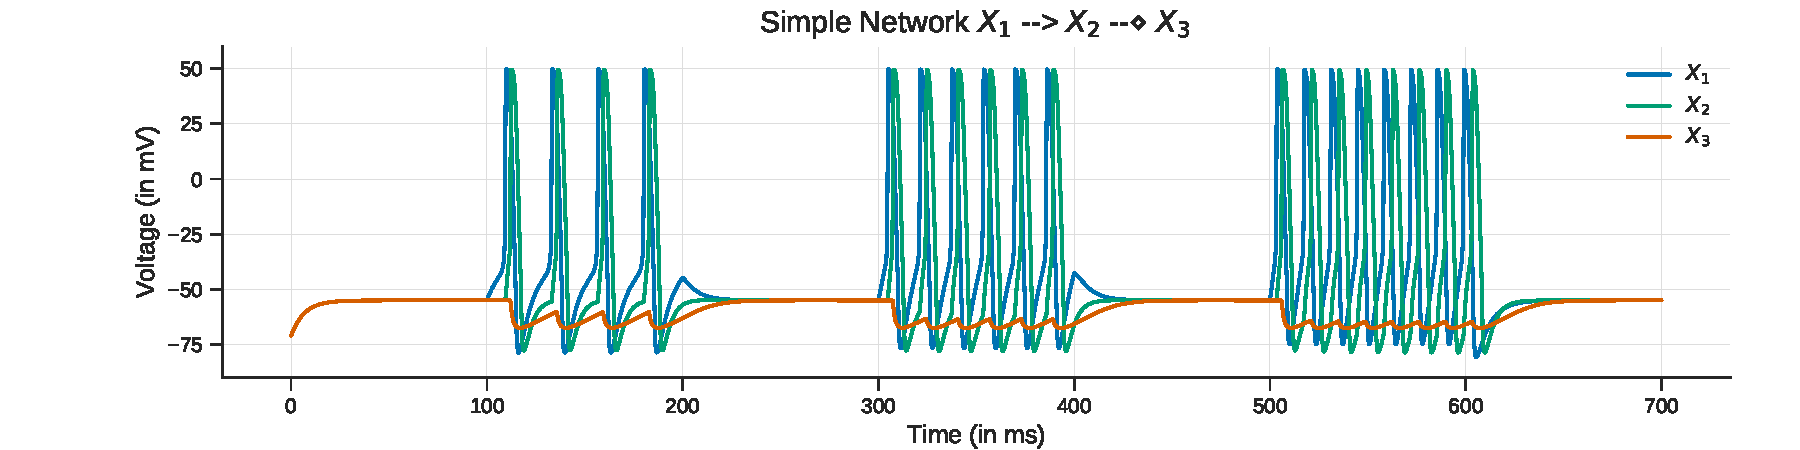
\includegraphics[scale=0.4]{Figures/fig13.pdf} 
%\caption{Pulses of current trigger the firing of action potentials with increasing frequency. Neuron $X_1$ crosses its firing threshold first and triggers neuron $X_2$ to fire after a slight delay. Finally, $X_{2}$ hyperpolarizes neuron $X_3$. 

\end{figure}

\end{center}

\section*{Day 5: Memory management}
Now that we can simulate a model network of conductance-based neurons, we discuss the limitations of our programs and our attempts to work around these issues.

\subsection*{Limits on memory}

Using Python and TensorFlow allowed us to write code that is readable, parallizable and scalable across a variety of computational devices. However, our implementation is very memory intensive. The iterators in TensorFlow do not follow the normal process of memory allocation and garbage collection. Since, TensorFlow is designed to work on diverse hardware like GPUs, TPUs and distributed platforms, memory allocation is done adaptively during the TensorFlow session and NOT cleared until the Python kernel has stopped execution. The memory used increases linearly with time as the state matrix is computed recursively by the \texttt{tf.scan} function. The maximum memory used by the computational graph is 2 times the total state matrix size at the point when the computation finishes and copies the final data into the memory. The larger the network and longer the simulation, the larger the solution matrix. Each run is limited by the total available memory. For a system with a limited memory of K bytes, The length of a given simulation (L timesteps) of a given network (N differential equations) with 64-bit floating-point precision will follow: 

\begin{eqnarray}2\times64\times L\times N=K\end{eqnarray}

That is, for any given network, our maximum simulation length is limited. One way to improve our maximum length is to divide the simulation into smaller batches. There will be a small queuing time between batches, which will slow down our code but will allow longer simulation times. Thus, if we split the simulation into K sequential batches, the maximum memory for the simulation becomes $(1+\frac{1}{K})$ times the total matrix size. Thus the memory relation becomes:  

\begin{eqnarray}\Big(1+\frac{1}{K}\Big)\times64\times L\times N=K\end{eqnarray}

This way, we can maximize the length of out simulation that we can run in a single Python kernel.

\subsection*{Implementing the Model}

To improve the readability of our code we separate the integrator into a independent import module. The integrator code was placed in a file called \texttt{tf\_integrator.py}. The file must be present in the same directory as the implementation of the model. 

Note: If you are using Jupyter Notebook, remember to remove the \%matplotlib inline command as it is specific to jupyter.

\subsubsection*{Importing tf\_integrator and other requirements}

Once the integrator, \texttt{tf\_integrator.py}, is saved in the same directory as the Notebook, we can start importing required libraries and the integrator.

\begin{minted}[linenos]{python}
import tensorflow as tf
import numpy as np
import tf_integrator as tf_int
import matplotlib.pyplot as plt
import seaborn as sns
\end{minted}

To simulate the code in batches we do not need to change how we construct our model only how we execute it.

\subsubsection*{Splitting time series into independent batches and run each batch sequentially}

Since we will be dividing the computation into batches, we have to split the time array such that for each new call, the final state vector of the last batch will be the initial condition for the current batch. The function \texttt{np.array\_split()} splits the array into non-overlapping vectors. Therefore, we append the last time of the previous batch to the beginning of the current time array batch.

\begin{minted}[linenos]{python}
# Define the Number of Batches
n_batch = 2
# Split t array into batches using numpy
t_batch = np.array_split(t,n_batch)
# Iterate over the batches of time array
for n,i in enumerate(t_batch):
    # Inform start of Batch Computation
    print("Batch",(n+1),"Running...",end="")
    # Re-adjusting edges
    if n>0:
        i = np.append(i[0]-sim_res,i)
    # Set state_vector as the initial condition
    init_state = tf.constant(state_vector, dtype=tf.float64)
    # Create the Integrator computation graph
    tensor_state = tf_int.odeint(dXdt, init_state, i, n_n, F_b)
    # Initialize variables and run session
    with tf.Session() as sess:
        tf.global_variables_initializer().run()
        state = sess.run(tensor_state)
        sess.close()
    # Reset state_vector as the last element of output
    state_vector = state[-1,:]
    # Save the output of the simulation to a binary file
    np.save("part_"+str(n+1),state)
    # Clear output
    state=None
    print("Finished")
\end{minted}

\subsubsection*{Putting the output together}

The output from our batch implementation is a set of binary files that store parts of our total simulation. To get the overall output we have to stitch them back together.

\begin{minted}[linenos]{python}
overall_state = []
# Iterate over the generated output files
for n,i in enumerate(["part_"+str(n+1)+".npy" for n in range(n_batch)]):
    # Since the first element in the series was the last output, 
    # we remove them
    if n>0:
        overall_state.append(np.load(i)[1:,:])
    else:
        overall_state.append(np.load(i))
# Concatenate all the matrix to get a single state matrix
overall_state = np.concatenate(overall_state)
\end{minted}

By this method, we have maximized the usage of our available memory. We can extend this further and develop a method to allow longer simulations. Since the memory is not cleared until the Python kernel finishes we save the parameters of the model (such as connectivity matrix) and the state vector in a file, and start a new Python kernel from a Python script to compute successive batches. This way after each large batch, the memory gets cleaned. By combining the previous batch implementation and this system, we can maximize our ability to run memory intensive simulations.

\subsection*{Implementing a Runner and a Caller}

First, we have to create an implementation of the model that takes in previous inputs as current parameters. Thus, we create a file, which we call \texttt{run.py} that takes an argument - the current batch number. The implementation for \texttt{run.py} is nearly the same as the previous code but with one minor difference. When the batch number is 0, we initialize all variable parameters and save them, otherwise we use the saved values. The parameters we save include the acetylcholine matrix, the GABA$_{A}$ matrix and the final/initial state vector. \texttt{run.py} also saves the files with both batch number and sub-batch number listed. 

\subsubsection*{Implementing the Caller code}
The caller function, \texttt{call.py} creates the time array, splits it into batches and uses the Python subprocess module to call \texttt{run.py} with appropriate arguments. The code for \texttt{call.py} is given below.

\begin{minted}[linenos]{python}
from subprocess import call
import numpy as np
total_time = 1000
n_splits = 2
time = np.split(np.arange(0,total_time,0.01),n_splits)
# Append the last time point to the beginning of the next batch
for n,i in enumerate(time):
    if n>0:
        time[n] = np.append(i[0]-0.01,i)
np.save("time",time)
# call successive batches with a new python subprocess 
# and pass the batch number
for i in range(n_splits):
    call(['python','run.py',str(i)])
print("Simulation Completed.")
\end{minted}

\subsubsection*{Implementing the Runner code}

\texttt{run.py} is essentially identical to the batch implementation we developed earlier with the changes described below.

\begin{minted}[linenos]{python}
# Additional Imports #
import sys
# Duration of Simulation #
# Replace t = np.arange(0,sim_time,sim_res) by
t = np.load("time.npy")[int(sys.argv[1])] # get first argument to run.py
# Connectivity Matrix Definitions #
if sys.argv[1] == '0':
    ach_mat = np.zeros((n_n,n_n)) # Ach Synapse Connectivity Matrix
    ach_mat[1,0]=1
    # If connectivity is random, once initialized it will be the same.
    np.save("ach_mat",ach_mat)
else:
    ach_mat = np.load("ach_mat.npy")
if sys.argv[1] == '0':
    gaba_mat = np.zeros((n_n,n_n)) # GABAa Synapse Connectivity Matrix
    gaba_mat[2,1] = 1
    # If connectivity is random, once initialized it will be the same.
    np.save("gaba_mat",gaba_mat)
else:
    gaba_mat = np.load("gaba_mat.npy")
# Current Input Definition #
if sys.argv[1] == '0':
    current_input= np.zeros((n_n,int(sim_time/sim_res)))
    current_input[0,int(100/sim_res):int(200/sim_res)] = 2.5
    current_input[0,int(300/sim_res):int(400/sim_res)] = 5.0
    current_input[0,int(500/sim_res):int(600/sim_res)] = 7.5
    np.save("current_input",current_input)
else:
    current_input = np.load("current_input.npy")
# State Vector Definition #
if sys.argv[1] == '0':
    state_vector = [-71]*n_n+[0,0,0]*n_n+[0]*n_ach+[0]*n_gaba
    						+[-9999999]*n_n
    state_vector = np.array(state_vector)
    state_vector = state_vector + 0.01*state_vector
    			*np.random.normal(size=state_vector.shape)
    np.save("state_vector",state_vector)
else:
    state_vector = np.load("state_vector.npy")
# Saving of Output #
# Replace np.save("part_"+str(n+1),state) by
np.save("batch"+str(int(sys.argv[1])+1)+"_part_"+str(n+1),state)
\end{minted}

\subsubsection*{Combining all Data}
Just as we merged all the batches, we merge all the sub-batches and batches.

\begin{minted}[linenos]{python}
overall_state = []
# Iterate over the generated output files
for n,i in enumerate(["batch"+str(x+1) for x in range(n_splits)]):
    for m,j in enumerate(["_part_"+str(x+1) for x in range(n_batch)]):
        # Since the first element in the series was the last output, 
        # we remove them
        if n>0 and m>0:
            overall_state.append(np.load(i+j+".npy")[1:,:])
        else:
            overall_state.append(np.load(i+j+".npy"))
# Concatenate all the matrix to get a single state matrix
overall_state = np.concatenate(overall_state)
\end{minted}

\section*{Conclusion}
The TensorFlow ecosystem is a rapidly evolving. This will imply that new functions that expand the use of TensorFlow. We anticipate that the code described here will serve as a starting point to simulate ODEs and could potentially evolve to include more sophisticated and faster integration algorithms and methods to manage limitations imposed by memory. 

\section*{Supporting information}
The code in this tutorial is implemented as a series of Python notebooks that can be downloaded from the following Github repository \texttt{https://github.com/technosap/PSST}. 
\section*{Acknowledgments}
SSM received a KVPY fellowship and support from IISER Pune. CA was funded by DBT–Wellcome India Alliance through an Intermediate fellowship IA/I/11/2500290 and IISER Pune. We thank members of the Assisi and Nadkarni labs at IISER Pune and several students who tested the code.  We thank Prof. Maxim Bazhenov for discussions and code related to the insect antennal lobe model.

\nolinenumbers
\bibliography{nerveFlow}
% Either type in your references using

% \bibitem{}
% Text
% \end{thebibliography}
%
% or
%
% Compile your BiBTeX database using our plos2015.bst
% style file and paste the contents of your .bbl file
% here. See http://journals.plos.org/plosone/s/latex for 
% step-by-step instructions.
% 
%\begin{thebibliography}{10}
%
%\bibitem{bib1}
%Conant GC, Wolfe KH.
%\newblock {{T}urning a hobby into a job: how duplicated genes find new
%  functions}.
%\newblock Nat Rev Genet. 2008 Dec;9(12):938--950.
%
%\bibitem{bib2}
%Ohno S.
%\newblock Evolution by gene duplication.
%\newblock London: George Alien \& Unwin Ltd. Berlin, Heidelberg and New York:
%  Springer-Verlag.; 1970.
%
%\bibitem{bib3}
%Magwire MM, Bayer F, Webster CL, Cao C, Jiggins FM.
%\newblock {{S}uccessive increases in the resistance of {D}rosophila to viral
%  infection through a transposon insertion followed by a {D}uplication}.
%\newblock PLoS Genet. 2011 Oct;7(10):e1002337.
%
%\end{thebibliography}



\end{document}

